\documentclass[fleqn]{article}
\oddsidemargin 0.0in
\textwidth 6.0in
\thispagestyle{empty}
\usepackage{import}
\usepackage{amsmath}
\usepackage[backend=bibtex]{biblatex}
\usepackage[utf8]{inputenc}
\usepackage{csquotes}
\usepackage{graphicx}
\usepackage{flexisym}
\usepackage{calligra}
\usepackage{amssymb}
\usepackage{bigints} 
\usepackage[english]{babel}
\usepackage{float}
\usepackage[colorinlistoftodos]{todonotes}
\usepackage{blindtext}
\usepackage{hyperref}

\addbibresource{references.bib}

\hypersetup{
  colorlinks=true,
  linkcolor=blue,
  filecolor=magenta,      
  urlcolor=cyan,
  pdfpagemode=FullScreen
}

\DeclareMathAlphabet{\mathcalligra}{T1}{calligra}{m}{n}
\DeclareFontShape{T1}{calligra}{m}{n}{<->s*[2.2]callig15}{}
\newcommand{\scriptr}{\mathcalligra{r}\,}
\newcommand{\boldscriptr}{\pmb{\mathcalligra{r}}\,}

\definecolor{red}{HTML}{F30000}

\setlength{\arrayrulewidth}{0.5mm}
\setlength{\tabcolsep}{18pt}
\renewcommand{\arraystretch}{1.5}


\begin{document}

  \begin{titlepage}

    \newcommand{\HRule}{\rule{\linewidth}{0.5mm}}

    \center

    \begin{center}
      
\includegraphics[height=11cm, width=11cm]{asu.png}
    \end{center}

    \vline

    \HRule \\[0.5cm]
    { \huge \bfseries Particle Collisions In The Universe}\\[0.4cm] 
    \HRule \\[1.0cm]

    \textbf{Behnam Amiri}

    \bigbreak

    \textbf{Prof: Cecilia Lunardini}

    \bigbreak

    \textbf{{\large \today}\\[2cm]}

    \vfill

  \end{titlepage}

  \textbf{What is an elastic collision?}

  \vspace{10px}

  An elastic collision is a collision in which there is no net loss in kinetic energy in the system as a result of 
  the collision. Both momentum and kinetic energy are conserved quantities in elastic collisions. Let's take a look 
  at two-dimensional elastic collision between two billiard balls. Imagine a billiard ball that is going to strike 
  another ball that is stationary. (The target is initially at rest)
  \begin{center}
    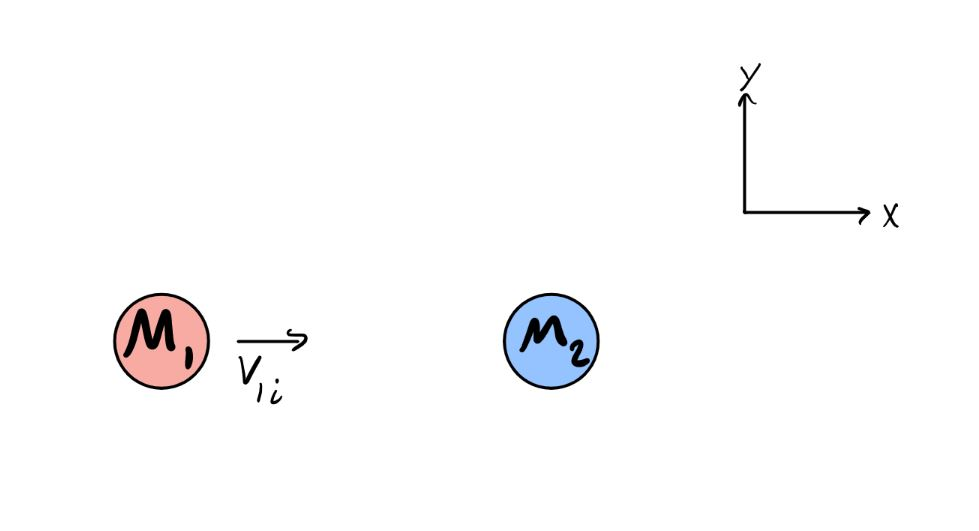
\includegraphics[height=4cm, width=7cm]{1.JPG}
  \end{center}

  Once the first ball hits the second ball, then they both go at different angles.

  \begin{center}
    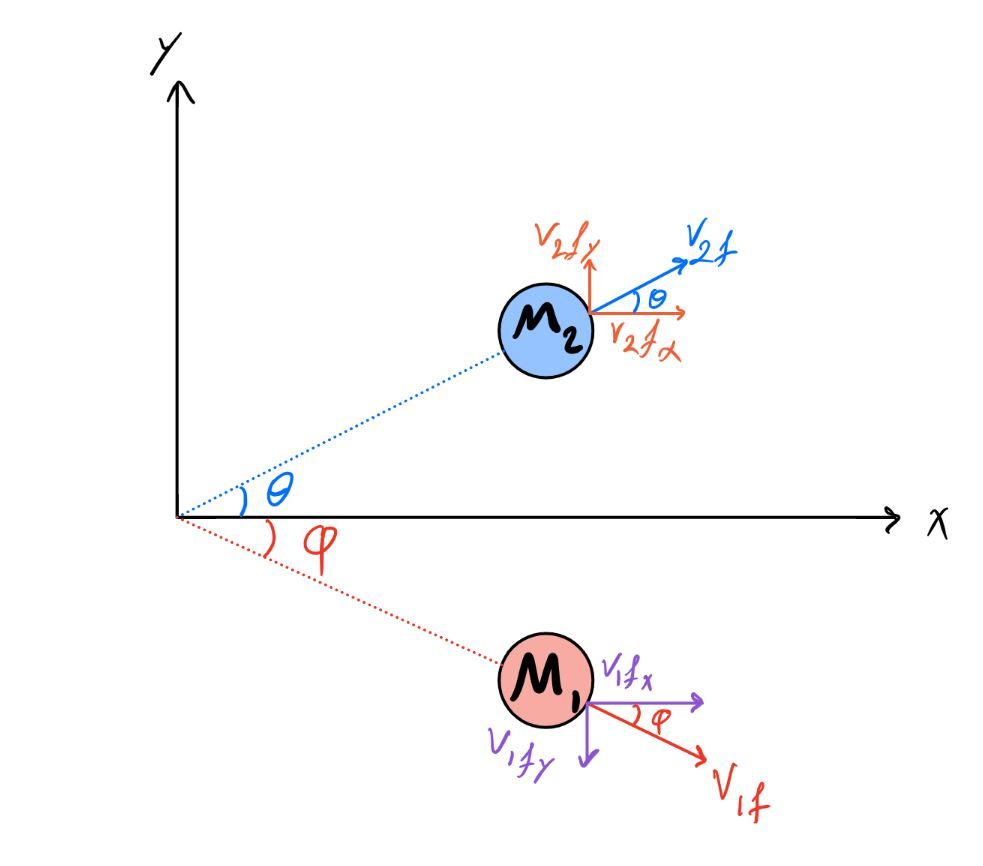
\includegraphics[height=8cm, width=10cm]{2.JPG}
  \end{center}

  \textbf{Elastic collision of balls with the same mass}

  \vspace{10px}

  Let's see how we can set up conservation of momentum. Since this is a elastic collision that means
  we also have conservation of kinetic energy.

  $
    \\
    \text{Momentum in the x-direction} ~~~ M_1 ~ v_{1i}=M_1 ~ v_{1f} ~ cos(\phi)+M_2 ~ v_{2f} ~ cos(\theta) ~~~~ (1)
    \\
    \\
    \text{Momentum in the y-direction} ~~~ 0=-M_1 ~ v_{1f} ~ sin(\phi)+M_2 ~ v_{2f} ~ sin(\theta) ~~~~~~~~~~~ (2)
  $

  \pagebreak

  Conservation of kinetic energy allows us to have:

  $
    \\
    \dfrac{1}{2} M_1 ~ v_{1i}^2=\dfrac{1}{2} M_1 ~ v_{1f}^2+\dfrac{1}{2} M_2 ~ v_{2f}^2 ~~~~~~~~ (3)
  $

  \vspace{10px}

  Assume the two balls have the same mass equals to $M_1=M_2=M$. Then we can rewrite equations $(1), (2),$ and $(3)$.

  $
    \\
    \begin{cases}
      v_{1i}=v_{1f} ~ cos(\phi)+v_{2f} ~ cos(\theta) ~~~~~~~~ (4)
      \\
      \\
      0=-v_{1f} sin(\phi)+v_{2f} ~ sin(\theta) ~~~~~~~~ (5)
      \\
      \\
      v_{1i}^2=v_{1f}^2+v_{2f}^2 ~~~~~~~~ (6)
    \end{cases}
    \\
    \\
  $

  Squaring $(4)$ and $(5)$ gives us:

  $
    \\
    \begin{cases}
      v_{1i}^2=v_{1f}^2 ~ cos^2(\phi)+v_{2f}^2 ~ cos^2(\theta)+2 v_{1f} ~ v_{2f} ~ cos(\phi) ~ cos(\theta) ~~~~~~~~ (7)
      \\
      \\
      0=v_{1f}^2 sin^2(\phi)+v_{2f}^2 ~ sin^2(\theta)-2 v_{1f} ~ v_{2f} ~ sin(\theta) ~ sin(\phi) ~~~~~~~~ (8)
    \end{cases}
    \\
    \\
  $

  By adding both equations $(7)$ and $(8)$ we get:

  $
    \\
    v_{1i}^2=v_{1f}^2 \left[sin^2(\phi)+cos^2(\phi)\right]+v_{2f}^2 \left[sin^2(\theta)+cos^2(\theta)\right]
    +2 v_{1f} ~ v_{2f} ~ \left[cos(\phi) ~ cos(\theta)-sin(\phi) ~ sin(\theta)\right]
    \\
    \\
    v_{1i}^2=v_{1f}^2+v_{2f}^2+2 v_{1f} ~ v_{2f} ~ \left[cos(\phi) ~ cos(\theta)-sin(\phi) ~ sin(\theta)\right]
    \\
    \\
  $

  Using $\boxed{cos(\phi+\theta)=cos(\phi) ~ cos(\theta)-sin(\phi) sin(\theta)}$ identity we have:

  $
    \\
    \\
    \therefore ~~~ v_{1i}^2=v_{1f}^2+v_{2f}^2+2 v_{1f} ~ v_{2f} ~ cos(\phi+\theta) ~~~~~~~~ (9)
    \\
    \\
  $

  From equations $(6)$ and $(9)$:

  $
    \\
    \begin{cases}
      v_{1i}^2=v_{1f}^2+v_{2f}^2+2 v_{1f} ~ v_{2f} ~ cos(\phi+\theta)
      \\
      \\
      v_{1i}^2=v_{1f}^2+v_{2f}^2
    \end{cases}
    \Longrightarrow
    v_{1f}^2+v_{2f}^2=v_{1f}^2+v_{2f}^2+2 v_{1f} ~ v_{2f} ~ cos(\theta+\phi)
    \\
    \\
    \\
    \therefore ~~~ \boxed{\theta+\phi=\dfrac{\pi}{2}} ~~~~ \checkmark
    \\
    \\
  $

 For a two dimensional collision where the balls have the same mass, \emph{billiard balls}, they always scatter 
 off at $\dfrac{\pi}{2}$ with each other. In other words, the angle between the two balls after the collision is
 always $\dfrac{\pi}{2}$ when they have the same mass.
 
 $
    \\
    \begin{cases}
      v_{1i}=v_{1f} ~ cos(\phi)+v_{2f} ~ cos(\theta) ~~~~~~~~ (4)
      \\
      \\
      0=-v_{1f} sin(\phi)+v_{2f} ~ sin(\theta) ~~~~~~~~ (5)
    \end{cases} 
    \Longrightarrow 
    \begin{cases}
      v_{1f}=\dfrac{
        \begin{vmatrix}
          v_{1i} & cos(\theta)
          \\
          0 & sin(\theta)
        \end{vmatrix}
      }{
        \begin{vmatrix}
          cos(\phi) & cos(\theta)
          \\
          -sin(\phi) & sin(\theta)
        \end{vmatrix}
      }
      \\
      \\
      v_{2f}=\dfrac{
        \begin{vmatrix}
          cos(\phi) & v_{1i}
          \\
          -sin(\phi) & 0
        \end{vmatrix}
      }{
        \begin{vmatrix}
          cos(\phi) & cos(\theta)
          \\
          -sin(\phi) & sin(\theta)
        \end{vmatrix}
      }
    \end{cases}
    \\
    \\
    \\
    \boxed{sin(\phi+\theta)=cos(\phi) ~ sin(\theta)+sin(\phi) ~ cos(\theta)}
    \\
    \\
    \\
    \therefore ~~~ \begin{cases}
      v_{1f}=v_{1i} \dfrac{sin(\theta)}{sin(\phi+\theta)}
      \\
      \\
      v_{2f}=v_{1i} \dfrac{sin(\phi)}{sin(\phi+\theta)}
    \end{cases} ~~~~ \checkmark
    \\
    \\
 $

 \vspace{20px}

\textbf{Elastic collision of balls with different masses}

\vspace{10px}

Let's study the case where the masses of the balls are not the same $M_1 \neq M_2$. Our case is an elastic collision
which means both momentum and kinetic energy are conserved. 

$
  \\
  \\
  \begin{cases}
    M_1 ~ v_{1i}=M_1 ~ v_{1f}+M_2 ~ v_{2f}  
    \\
    \\
    \dfrac{1}{2} M_1 ~ v_{1i}^2=\dfrac{1}{2} M_1 ~ v_{1f}^2+\dfrac{1}{2} M_2 ~ v_{2f}^2  
  \end{cases}
  \Longrightarrow 
  \begin{cases}
    M_1 ~ v_{1i}=M_1 ~ v_{1f}+M_2 ~ v_{2f}
    \\
    \\
    M_1 ~ v_{1i}^2=M_1 ~ v_{1f}^2+M_2 ~ v_{2f}^2
  \end{cases}
  \\
  \\
  \\
  \\
  \begin{cases}
    M_1 ~ v_{1i}-M_1 ~ v_{1f}=M_2 ~ v_{2f}
    \\
    \\
    M_1 ~ v_{1i}^2-M_1 ~ v_{1f}^2=M_2 ~ v_{2f}^2
  \end{cases}
  \Longrightarrow
  \begin{cases}
    M_1\left(v_{1i}-v_{1f}\right)=M_2 ~ v_{2f} ~~~~~~~~ (A)
    \\
    \\
    M_1 ~ \left(v_{1i}-v_{1f}\right) ~ \left(v_{1i}+v_{1f}\right)=M_2 ~ v_{2f}^2 ~~~~~~~~ (B)
  \end{cases}
  \\
  \\
$

Dividing $(A)$ and $(B)$ gives us $\dfrac{1}{v_{1i}+v_{1f}}=\dfrac{1}{v_{2f}} \Longrightarrow v_{1i}+v_{1f}=v_{2f} ~~~~~ (C)$.
Now we can eliminate $v_{2f}$ by substituting $(C)$ into equation $(A)$.

$
  \\
  M_1\left(v_{1i}-v_{1f}\right)=M_2 ~ v_{2f}
  \Longrightarrow
  M_1\left(v_{1i}-v_{1f}\right)=M_2 ~ \left[v_{1i}+v_{1f}\right]
  \\
  \\
  M_1 ~ v_{1i}-M_1 ~ v_{1f}=M_2 ~ v_{1i}+M_2 ~ v_{1f} 
  \Longrightarrow 
  M_1 ~ v_{1i}-M_2 ~ v_{1i}=M_1 ~ v_{1f}+M_2 ~ v_{1f}
  \\
  \\
  \\
  \therefore ~~~ \boxed{v_{1f}=v_{1i} ~ \dfrac{M_1 - M_2}{M_1+M_2}} ~~~~ \checkmark
  \\
  \\
$

Time to eliminate $v_{1f}$, again by using $(C)$ and $(A)$. So we have

$
  \\
  M_1\left(v_{1i}-v_{1f}\right)=M_2 ~ v_{2f} 
  \Longrightarrow  M_1 \left[v_{1i}-\left(v_{2f}-v_{1i}\right)\right]=M_2 ~ v_{2f}
  \\
  \\
  M_1 \left[2v_{1i}-v_{2f}\right]=M_2 ~ v_{2f} \Longrightarrow 2 M_1 ~ v_{1i}=M_1 ~ v_{2f}+M_2 ~ v_{2f}
  \\
  \\
  \\
  \therefore ~~~ \boxed{v_{2f}=2 v_{1i} \dfrac{M_1}{M_1+M_2}} ~~~~ \checkmark
  \\
  \\
$

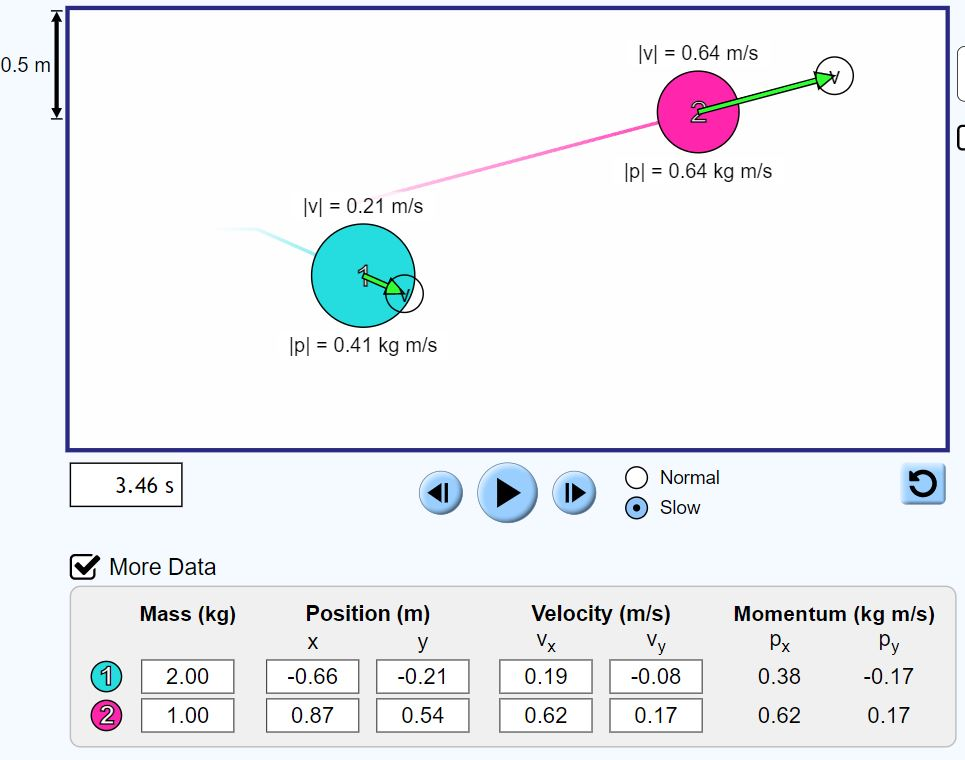
\includegraphics[height=6cm, width=10cm]{14.JPG}

$
  \\
  \begin{cases}
    M_1=2 ~ kg
    \\
    \\
    M_2=1 ~ kg
    \\
    \\
    V_i=0.5 ~ m/s
    \\
    \\
  \end{cases} \Longrightarrow 
  \boxed{
    \begin{cases}
      v_{1f}=v_{1i} ~ \dfrac{M_1 - M_2}{M_1+M_2}
      =0.5 ~ \dfrac{2 - 1}{2+1}=0.1666
      \\
      \\
      v_{2f}=2 v_{1i} \dfrac{M_1}{M_1+M_2}
      =2 (0.5) \dfrac{2}{2+1}=0.65
    \end{cases}
  } ~~~~ \checkmark
$

\pagebreak

We would like to know when the energy of the second ball is the largest. We are trying to find the maximum amount 
of kinetic energy of the first ball of mass $M_1$ which we can transfer to the second ball of mass $M_2$. We are considering 
the maximum kinetic energy of the first ball to be transferred to the second ball. By conservation of energy and momentum we have

$
  \\
  \begin{cases}
    M_1 ~ v_{1i}=M_1 ~ v_{1f}+M_2 ~ v_{2f}  
    \\
    \\
    \dfrac{1}{2} M_1 ~ v_{1i}^2=\dfrac{1}{2} M_1 ~ v_{1f}^2+\dfrac{1}{2} M_2 ~ v_{2f}^2  
  \end{cases}
  \\
  \\
$

When $v_{1f}=0$, then $100\%$ of the kinetic energy of the first ball must be transferred to the second ball in our case 
which is an elastic collision.

$
  \\
  \begin{cases}
    M_1 ~ v_{1i}=0+M_2 ~ v_{2f}  
    \\
    \\
    M_1 ~ v_{1i}^2=0+M_2 ~ v_{2f}^2  
  \end{cases} 
  \Longrightarrow 
  \left(\dfrac{M_1}{M_2} v_{1i} \right)^2=\dfrac{M_1}{M_2} v_{1i}^2
  \Longrightarrow \dfrac{M_1}{M_2}=1
  \\
  \\
  \\
  \therefore ~~~ \boxed{M_1=M_2} ~~~~ \checkmark
  \\
$

\pagebreak

\textbf{Non-head-on elastic collision of balls with different masses (1)}

\vspace{10px}

A head-on collision is a traffic collision where the front ends of two vehicles such as cars, trains, ships or planes 
hit each other when travelling in opposite directions, as opposed to a side collision or rear-end collision.
A head on collision means that the point of impact is on the straight line connecting the center of gravity of each of 
the objects. The centres of mass of the two bodies should be travelling in the same straight line and approaching each other 
to call it a head on collision.

\begin{center}
  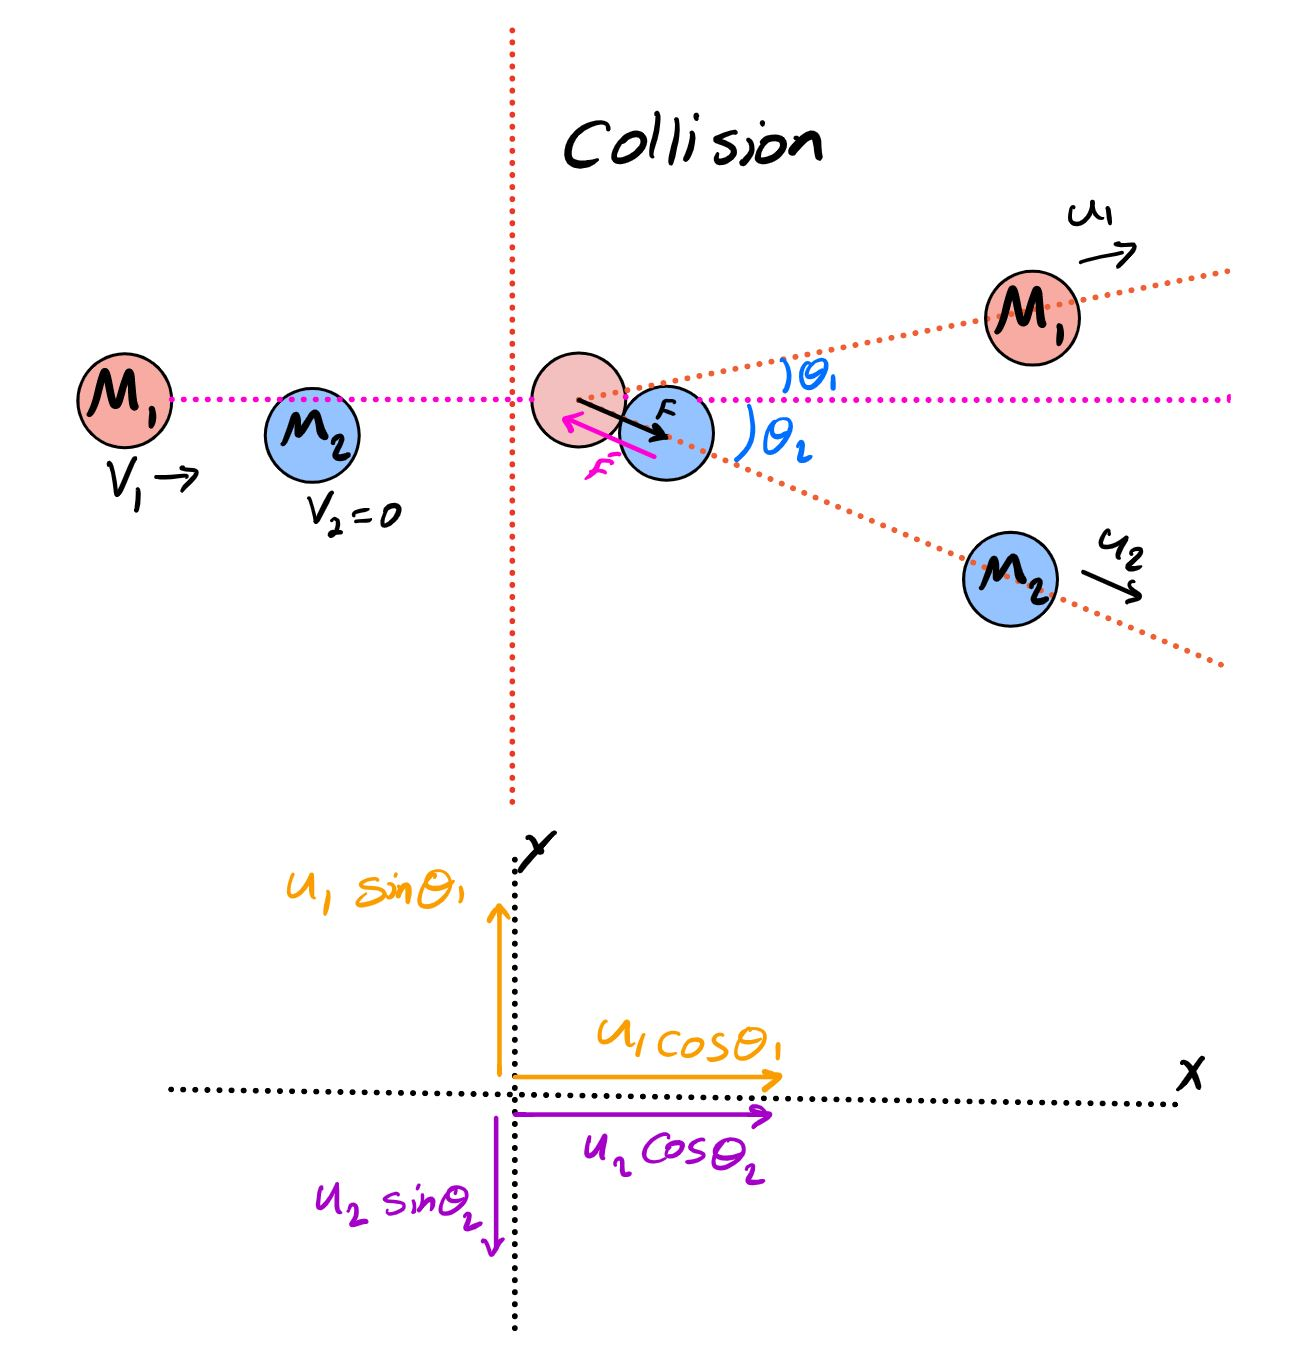
\includegraphics[height=11cm, width=10cm]{3.JPG}
\end{center}

$
  \\
  \text{Momentum in the x-direction (conserved)} ~~~ (I): ~~~ m_1 ~ v_{1}+0=m_1 ~ u_1 ~ cos(\theta_1)+m_2 ~ u_2 ~ cos(\theta_2)
  \\
  \\
  \text{Momentum in the y-direction (conserved)} ~~~ (II): ~~~ 0=m_1 ~ u_1 ~ sin(\theta_1)-m_2 ~ u_2 ~ sin(\theta_2)
  \\
  \\
  \text{Kinetic energy (conserved and scalar quantity)} ~~~ (III): 
  \dfrac{1}{2} m_1 ~ v^2_1+0=\dfrac{1}{2} m_1 ~ u^2_1+\dfrac{1}{2} m_2 ~ u^2_2
$

\vspace{10px}

We have got three equations meaning we only can find 3 unknown variables. Assuming we are given 
$m_1, m_2, v_1,$ and $u_1$ we can find $u_2, ~ \theta_1,$ and $\theta_2$. From equation $(III)$ we have

$
  \\
  m_1 ~ v^2_1=m_1 ~ u^2_1+m_2 ~ u^2_2
  \\
  \\
  \therefore ~~~ \dfrac{m_1}{m_2} \left(v_1^2-u_1^2\right)=u_2^2
  \\
  \\
  \\
  \therefore ~~~ \boxed{u_2=\sqrt{\dfrac{m_1}{m_2} \left(v_1^2-u_1^2\right)}} ~~~~ \checkmark
  \\
  \\
  \\
$

Now that we have $u_2$, we are able to find $\theta_1$ and $\theta_2$.

$
\\
  (IV): ~~~ \begin{cases}
    m_1 ~ u_1 ~ cos(\theta_1)+m_2 ~ u_2 ~ cos(\theta_2)=m_1 ~ v_{1}
    \\
    \\
    m_1 ~ u_1 ~ sin(\theta_1)-m_2 ~ u_2 ~ sin(\theta_2)=0
  \end{cases}
  \\
  \\
$

Squaring and summing $(IV)$ gives us

$
  \\
  \\
  m_1^2 ~ u_1^2 \left[cos^2(\theta_1)+sin^2(\theta_1)\right]=m_2^2 ~ u_2^2 ~ sin^2(\theta_2)
  +\left[m_1^2 ~ v_1^2+m_2^2 ~ u_2^2 ~ cos^2(\theta_2)-2m_1 ~ v_1 ~ m_2 ~ u_2 ~ cos(\theta_2)\right]
  \\
  \\
  m_1^2 ~ u_1^2=m_2^2 ~ u_2^2 ~ sin^2(\theta_2)+m_1^2 ~ v_1^2 +m_2^2 ~ u_2^2 ~ cos^2(\theta_2)-2m_1 ~ v_1 ~ m_2 ~ u_2 ~ cos(\theta_2)
  \\
  \\
  m_1^2 ~ u_1^2=m_2^2 ~ u_2^2 \left[sin^2(\theta_2)+cos^2(\theta_2)\right]+m_1^2 ~ v_1^2-2m_1 ~ v_1 ~ m_2 ~ u_2 ~ cos(\theta_2)
  \\
  \\
  m_1^2 ~ u_1^2=m_2^2 ~ u_2^2+m_1^2 ~ v_1^2-2m_1 ~ v_1 ~ m_2 ~ u_2 ~ cos(\theta_2)
  \\
  \\
  cos(\theta_2)=\dfrac{
    -m_1^2 ~ u_1^2+m_2^2 ~ u_2^2+m_1^2 ~ v_1^2 
  }{
    2 ~ m_1 ~ v_1 ~ m_2 ~ u_2
  }=\dfrac{
    m_1^2 ~ \left(v_1^2-u_1^2\right)+m_2^2 ~u_2^2 
  }{
    2 m_1 ~ m_2 ~ v_1 ~ u_2
  }
  \\
  \\
  \\
  \therefore ~~~ \boxed{
    \theta_2=cos^{-1}\left[
      \dfrac{
        m_1^2 ~ \left(v_1^2-u_1^2\right)+m_2^2 ~u_2^2 
      }{
        2 m_1 ~ m_2 ~ v_1 ~ u_2
      }
    \right]
  } ~~~~ \checkmark
$

\pagebreak

Using the same method as we used above to calculate $\theta_1$

$
  \\
  \\
  (IV): ~~~ \begin{cases}
    m_1 ~ u_1 ~ cos(\theta_1)+m_2 ~ u_2 ~ cos(\theta_2)=m_1 ~ v_{1}
    \\
    \\
    m_1 ~ u_1 ~ sin(\theta_1)-m_2 ~ u_2 ~ sin(\theta_2)=0
  \end{cases}
  \\
  \\
  \\
  \begin{cases}
    m_1 ~ u_1 ~ cos(\theta_1)-m_1 ~ v_{1}=-m_2 ~ u_2 ~ cos(\theta_2)
    \\
    \\
    m_1 ~ u_1 ~ sin(\theta_1)=m_2 ~ u_2 ~ sin(\theta_2)
  \end{cases}
  \\
  \\
  \\
  \begin{cases}
    m_1^2 ~ u_1^2 ~ cos^2(\theta_1)+m_1^2 ~ v_{1}^2-2 ~ m_1 ~ u_1 ~ m_1 ~ v_1 ~ cos(\theta_1)=m_2^2 ~ u_2^2 ~ cos^2(\theta_2)
    \\
    \\
    m_1^2 ~ u_1^2 ~ sin^2(\theta_1)=m_2^2 ~ u_2^2 ~ sin^2(\theta_2)
  \end{cases}
  \\
  \\
  \\
  m_1^2 ~ u_1^2 ~ cos^2(\theta_1)+m_1^2 ~ v_{1}^2-2 ~ m_1 ~ u_1 ~ m_1 ~ v_1 ~ cos(\theta_1)
  +m_1^2 ~ u_1^2 ~ sin^2(\theta_1)
  =m_2^2 ~ u_2^2 ~ cos^2(\theta_2)+m_2^2 ~ u_2^2 ~ sin^2(\theta_2)
  \\
  \\
  \\
  m_1^2 ~ u_1^2 ~ \left[cos^2(\theta_1)+sin^2(\theta_1)\right]+m_1^2 ~ v_1^2-2 ~ m_1 ~ u_1 ~ m_1 ~ v_1 ~ cos(\theta_1)
  =m_2^2 ~ u_2^2 ~ \left[cos^2(\theta_2)+sin^2(\theta_2)\right]
  \\
  \\
  \\
  m_1^2 ~ u_1^2+m_1^2 ~ v_1^2-2 ~ m_1 ~ u_1 ~ m_1 ~ v_1 ~ cos(\theta_1)
  =m_2^2 ~ u_2^2
  \\
  \\
  \\
  2 ~ m_1 ~ u_1 ~ m_1 ~ v_1 ~ cos(\theta_1)=m_1^2 ~ u_1^2+m_1^2 ~ v_1^2-m_2^2 ~ u_2^2
  \\
  \\
  \\
  cos(\theta_1)=\dfrac{m_1^2 \left(u_1^2+v_1^2\right)-m_2^2 ~ u_2^2}{2 ~ m_1^2 ~ u_1 ~ v_1}
  \\
  \\
  \\
  \therefore ~~~ \boxed{
    \theta_1=cos^{-1} \left[
      \dfrac{m_1^2 \left(u_1^2+v_1^2\right)-m_2^2 ~ u_2^2}{2 ~ m_1^2 ~ u_1 ~ v_1}
    \right]
  } ~~~~ \checkmark
  \\
  \\
$

Note: The domain and range of $y=cos^{-1}(x)$ are $-1 \leq x \leq +1$ and $0 \leq y \leq +\pi$. 

We know the kinetic energy of the second ball is 
$
  \\
  \\
  KE=\dfrac{1}{2} ~ m_2 ~ u_2^2=\dfrac{1}{2} ~ m_2 ~ \left[
    \sqrt{\dfrac{m_1}{m_2} \left(v_1^2-u_1^2\right)}
  \right]^2
  =\dfrac{1}{2} ~ m_2 ~ \dfrac{m_1}{m_2} \left(v_1^2-u_1^2\right)
  \\
  \\
  \\
  \therefore ~~~ \boxed{
    KE=\dfrac{1}{2} ~ m_1 \left(v_1^2-u_1^2\right)
  } ~~~~ \checkmark
  \\
  \\
$

Maximizing the energy transferred to the second ball? (Largest kinetic energy)

\vspace{10px}

\textbf{Some examples}

\vspace{10px}

$
  (A) ~ m_1=m_2=2 ~ kg, v_1=3 ~ m/s ~ , u_1=2 ~ m/s
  \\
  \\
  \begin{cases}
    u_2=\sqrt{\dfrac{m_1}{m_2} \left(v_1^2-u_1^2\right)}=\sqrt{\left(v_1^2-u_1^2\right)}=2.2360 ~ m/s
    \\
    \\
    \theta_1=cos^{-1} \left[
      \dfrac{m_1^2 \left(u_1^2+v_1^2\right)-m_2^2 ~ u_2^2}{2 ~ m_1^2 ~ u_1 ~ v_1}
    \right]=48.1896^{\circ}
    \\
    \\
    \theta_2=cos^{-1}\left[
      \dfrac{
        m_1^2 ~ \left(v_1^2-u_1^2\right)+m_2^2 ~u_2^2 
      }{
        2 m_1 ~ m_2 ~ v_1 ~ u_2
      }
    \right]=41.8103^{\circ}
  \end{cases} ~~~ \therefore ~~~ \boxed{\theta_1+\theta_2=\dfrac{\pi}{2}} ~~~~ \checkmark 
  \\
  \\
  \\
  (B) ~ m_1>m_2, ~ 5 ~ kg, ~ 4 ~ kg, ~ v_1=4 ~ m/s ~ , u_1=2 ~ m/s
  \\
  \\
  \begin{cases}
    u_2=\sqrt{\dfrac{m_1}{m_2} \left(v_1^2-u_1^2\right)}=3.8729 ~ m/s
    \\
    \\
    \theta_1=cos^{-1} \left[
      \dfrac{m_1^2 \left(u_1^2+v_1^2\right)-m_2^2 ~ u_2^2}{2 ~ m_1^2 ~ u_1 ~ v_1}
    \right]=49.4583^{\circ}
    \\
    \\
    \theta_2=cos^{-1}\left[
      \dfrac{
        m_1^2 ~ \left(v_1^2-u_1^2\right)+m_2^2 ~u_2^2 
      }{
        2 m_1 ~ m_2 ~ v_1 ~ u_2
      }
    \right]=29.3757^{\circ}
  \end{cases} 
  \\
  \\
  \\
  (C) ~ m_1<m_2, ~ 2 ~ kg, ~ 6 ~ kg, ~ v_1=2 ~ m/s ~ , u_1=1 ~ m/s
  \\
  \\
  \begin{cases}
    u_2=\sqrt{\dfrac{m_1}{m_2} \left(v_1^2-u_1^2\right)}=1 ~ m/s
    \\
    \\
    \theta_1=cos^{-1} \left[
      \dfrac{m_1^2 \left(u_1^2+v_1^2\right)-m_2^2 ~ u_2^2}{2 ~ m_1^2 ~ u_1 ~ v_1}
    \right]=180^{\circ}
    \\
    \\
    \theta_2=cos^{-1}\left[
      \dfrac{
        m_1^2 ~ \left(v_1^2-u_1^2\right)+m_2^2 ~u_2^2 
      }{
        2 m_1 ~ m_2 ~ v_1 ~ u_2
      }
    \right]=0^{\circ} 
  \end{cases}
$

\pagebreak

\textbf{Non-head-on elastic collision of balls with different masses (2)}

\vspace{10px}

A head-on collision is a traffic collision where the front ends of two vehicles such as cars, trains, ships or planes 
hit each other when travelling in opposite directions, as opposed to a side collision or rear-end collision.
A head on collision means that the point of impact is on the straight line connecting the center of gravity of each of 
the objects. The centres of mass of the two bodies should be travelling in the same straight line and approaching each other 
to call it a head on collision.

\begin{center}
  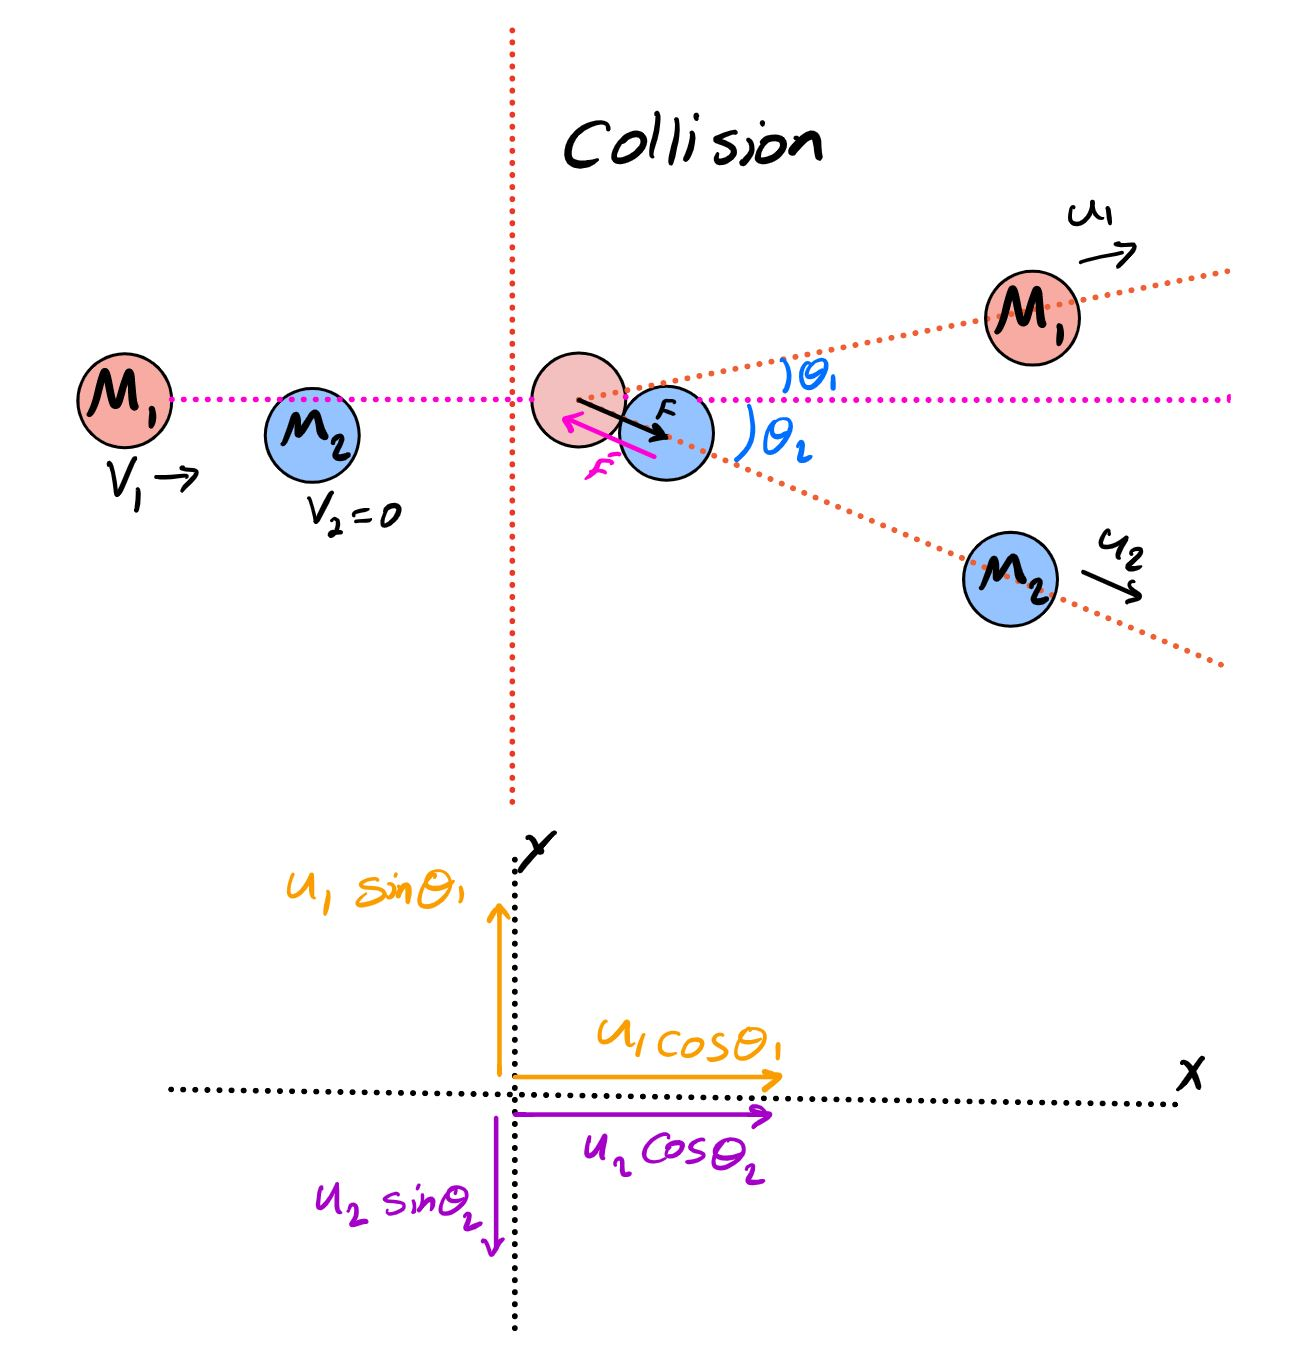
\includegraphics[height=11cm, width=10cm]{3.JPG}
\end{center}

$
  \\
  \text{Momentum in the x-direction (conserved)} ~~~ (I): ~~~ m_1 ~ v_{1}+0=m_1 ~ u_1 ~ cos(\theta_1)+m_2 ~ u_2 ~ cos(\theta_2)
  \\
  \\
  \text{Momentum in the y-direction (conserved)} ~~~ (II): ~~~ 0=m_1 ~ u_1 ~ sin(\theta_1)-m_2 ~ u_2 ~ sin(\theta_2)
  \\
  \\
  \text{Kinetic energy (conserved and scalar quantity)} ~~~ (III): 
  \dfrac{1}{2} m_1 ~ v^2_1+0=\dfrac{1}{2} m_1 ~ u^2_1+\dfrac{1}{2} m_2 ~ u^2_2
$

\pagebreak

$
  \\
  \begin{cases}
    (1): ~ m_1 ~ u_1 ~ cos(\theta_1)+m_2 ~ u_2 ~ cos(\theta_2)=m_1 ~ v_1
    \\
    \\
    (2): ~ m_1 ~ u_1 ~ sin(\theta_1)-m_2 ~ u_2 ~ sin(-\theta_2)=0 \Longrightarrow u_2=\dfrac{m_1 ~ u_1 ~ sin(\theta_1)}{m_2 ~ sin(-\theta_2)}
  \end{cases}
  \\
  \\
$

Plugging in $u_2$ into equation $(1)$ we get:

\vspace{10px}

$
  \\
  m_1 ~ u_1 ~ cos(\theta_1)+m_2 ~ \bigg(\dfrac{m_1 ~ u_1 ~ sin(\theta_1)}{m_2 ~ sin(-\theta_2)}\bigg) ~ cos(\theta_2)=m_1 ~ v_1
  \\
  \\
  \\
  m_1 ~ u_1 ~ cos(\theta_1)+\dfrac{m_1 ~ u_1 ~ sin(\theta_1)}{sin(-\theta_2)}~ cos(\theta_2)=m_1 ~ v_1
  \\
  \\
  \\
  u_1 ~ cos(\theta_1)+\dfrac{u_1 ~ sin(\theta_1)}{sin(-\theta_2)}~ cos(\theta_2)=v_1
  \\
  \\
  \\
  u_1 ~ \left[cos(\theta_1)+\dfrac{sin(\theta_1) ~ cos(\theta_2)}{sin(-\theta_2)}\right]=v_1
  \\
  \\
  \\
  cos(\theta_1)+\dfrac{sin(\theta_1) ~ cos(\theta_2)}{sin(-\theta_2)}=\dfrac{v_1}{u_1}
  \Longrightarrow
  \dfrac{sin(-\theta_2) ~ cos(\theta_1)+cos(\theta_2) ~ sin(\theta_1)}{sin(-\theta_2)}=\dfrac{v_1}{u_1}
  \\
  \\
  \\
  -sin(\theta_2) ~ cos(\theta_1)+cos(\theta_2) ~ sin(\theta_1)=-sin(\theta_2) \dfrac{v_1}{u_1}
  \\
  \\
  \\
  \therefore ~~~ \boxed{
    (3): ~ sin(\theta_2) ~ cos(\theta_1)-cos(\theta_2) ~ sin(\theta_1)=sin(\theta_2) \dfrac{v_1}{u_1}
  } ~~~~ \checkmark
  \\
  \\
$

In trigonometry we learned that $\mathbf{A} ~ cos(\theta)-\mathbf{B} ~ sin(\theta)=\mathbf{C} \equiv \mathbf{R} ~ cos(\theta+\alpha)$ 
where $\mathbf{R}=\sqrt{\mathbf{A}^2+\mathbf{B}^2}$ and $\alpha=tan^{-1} \left(\dfrac{\mathbf{B}}{\mathbf{A}}\right)$. So let's use this 
identity to solve eqution $(3)$.

\pagebreak

$
  \\
  \begin{cases}
    R=\sqrt{sin^2(\theta_2)+cos^2(\theta_2)}=1, ~~ \alpha=tan^{-1} \left(\dfrac{cos(\theta_2)}{sin(\theta_2)}\right)
    \\
    \\
    sin(\theta_2) ~ cos(\theta_1)-cos(\theta_2) ~ sin(\theta_1)=\mathbf{R} ~ cos(\theta_1+\alpha)=sin(\theta_2) \dfrac{v_1}{u_1}
  \end{cases}
  \\
  \\
  \\
  \Longrightarrow cos(\theta_1+\alpha)=sin(\theta_2) \dfrac{v_1}{u_1}
  \Longrightarrow \theta_1+\alpha=cos^{-1} \bigg(sin(\theta_2) \dfrac{v_1}{u_1}\bigg)
  \\
  \\
  \\
  \therefore ~ \theta_1=cos^{-1} \bigg(sin(\theta_2) \dfrac{v_1}{u_1}\bigg)-\alpha
  =cos^{-1} \bigg(sin(\theta_2) \dfrac{v_1}{u_1}\bigg)-tan^{-1} \bigg(\dfrac{cos(\theta_2)}{sin(\theta_2)}\bigg)
  \\
  \\
  \\
  \therefore ~~~ \boxed{
    (4): ~ \theta_1=cos^{-1} \bigg(sin(\theta_2) ~ \dfrac{v_1}{u_1}\bigg)-tan^{-1} \bigg(\dfrac{cos(\theta_2)}{sin(\theta_2)}\bigg)
  } ~~~~ \checkmark
  \\
  \\
$

Earlier we found $u_2$ and in order to find its value we needed the value of $\theta_1$. Now by knowing $\theta_1$ we can compute $u_2$. Equations 
$(1)$ and $(2)$ \emph{can be only used to find two unknowns}, so assuming we are given $m_1, m_2, v_1, u_1$ and $\theta_2$. We can find $u_2$, 
and $\theta_1$.

\vspace{10px}

$
  \\
  u_2=\dfrac{m_1 ~ u_1 ~ sin(\theta_1)}{m_2 ~ sin(-\theta_2)}
  =\dfrac{m_1 ~ u_1}{m_2 ~ sin(-\theta_2)} sin \bigg[ 
    cos^{-1} \bigg(sin(\theta_2) ~ \dfrac{v_1}{u_1}\bigg)-tan^{-1} \bigg(\dfrac{cos(\theta_2)}{sin(\theta_2)}\bigg)  
  \bigg]
  \\
  \\
  \\
  \therefore ~~~ \boxed{
    (5): ~ u_2=\dfrac{m_1 ~ u_1}{m_2 ~ sin(-\theta_2)} sin \bigg[ 
      cos^{-1} \bigg(sin(\theta_2) ~ \dfrac{v_1}{u_1}\bigg)-tan^{-1} \bigg(\dfrac{cos(\theta_2)}{sin(\theta_2)}\bigg)  
    \bigg]
  } ~~~~ \checkmark
$

\pagebreak

\textbf{Non-head-on elastic collision of balls with different masses (3)}

\textbf{(Using reference frame of the Center of Mass)}

\vspace{10px}

An object's \emph{center of mass} can be thought of as the point where the total mass of an object or a 
system is treated as a point mass. The center of mass of a system of particles is a specific point at 
which the system's mass behaves as if it were concentrated. 

Another way of expressing the \emph{center of mass} is a point where if whole of the mass of the body gets concentrated, 
and then the body is balanced at this point then it experiences no net torque and will remain in static equilibrium.

$$
  x_{cm}=\dfrac{
    \sum\limits_{i=1}^{n} ~ m_i ~ r_i
  }{
    \sum\limits_{i=1}^{n} ~ m_i
  } ~~~~~~~~~~~~
  v_{cm}=\dfrac{
    \sum\limits_{i=1}^{n} ~ p_i
  }{
    \sum\limits_{i=1}^{n} ~ m_i
  }
$$

A quick description of what the laboratory frame and center of mass references are. The \emph{laboratory frame} is a frame 
whereby positions and velocities are measured with respect to the laboratory and the \emph{center of mass} frame is a frame 
whereby the positions and velocities are measured with respect to the the center of mass of a system. Basically, we need 
to change to a moving coordinate system which goes with the velocity of the center of mass.\textbf{ The total momentum 
is always zero in the center of mass reference frame}.

\begin{center}
  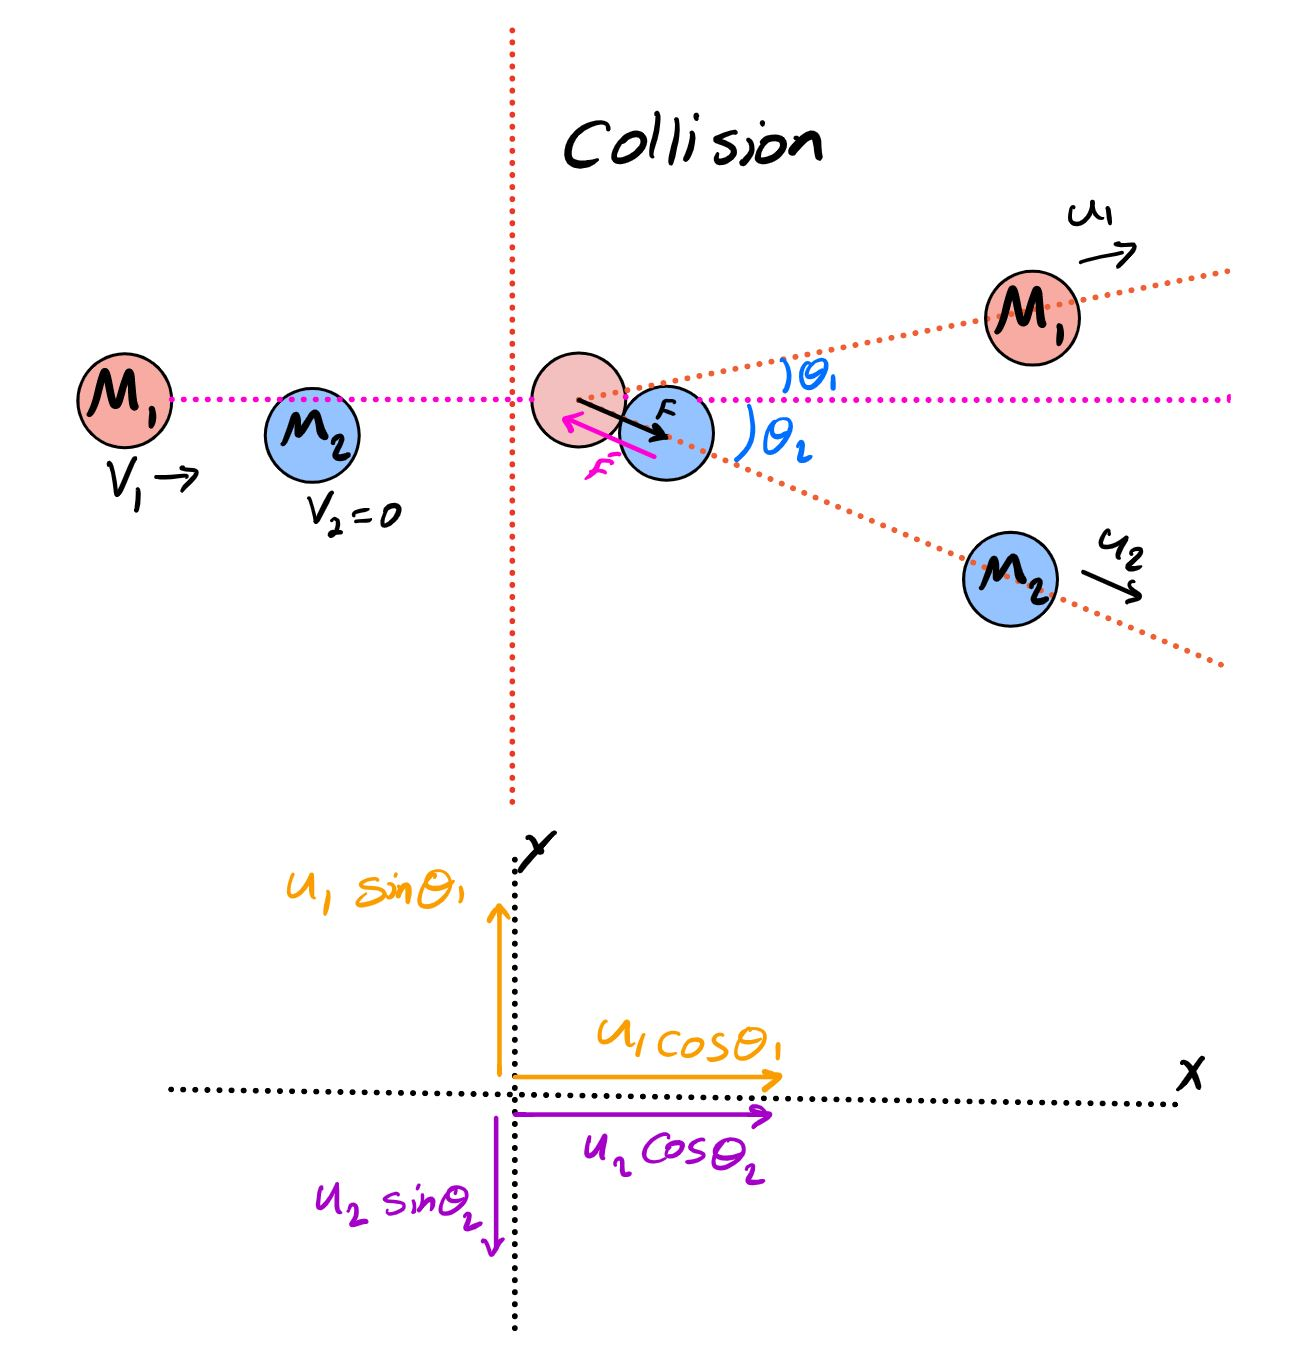
\includegraphics[height=10cm, width=9cm]{3.JPG}
\end{center}

In center of mass frame

$
  \\
  \begin{cases}
    x_{cm}=\dfrac{
      \sum\limits_{i=1}^{n} ~ m_i ~ r_i
    }{
      \sum\limits_{i=1}^{n} ~ m_i
    }=\dfrac{m_1 ~ x_1+m_2 ~ x_2}{m_1+m_2} ~ \hat{x}
    \\
    \\
    \\
    v_{cm}=\dfrac{
      \sum\limits_{i=1}^{n} ~ p_i
    }{
      \sum\limits_{i=1}^{n} ~ m_i
    }=\dfrac{m_1 ~ v_1+m_2 ~ v_2}{m_1+m_2}=\dfrac{m_1 ~ v_1}{m_1+m_2} ~ \hat{x}
  \end{cases}
$

\begin{center}
  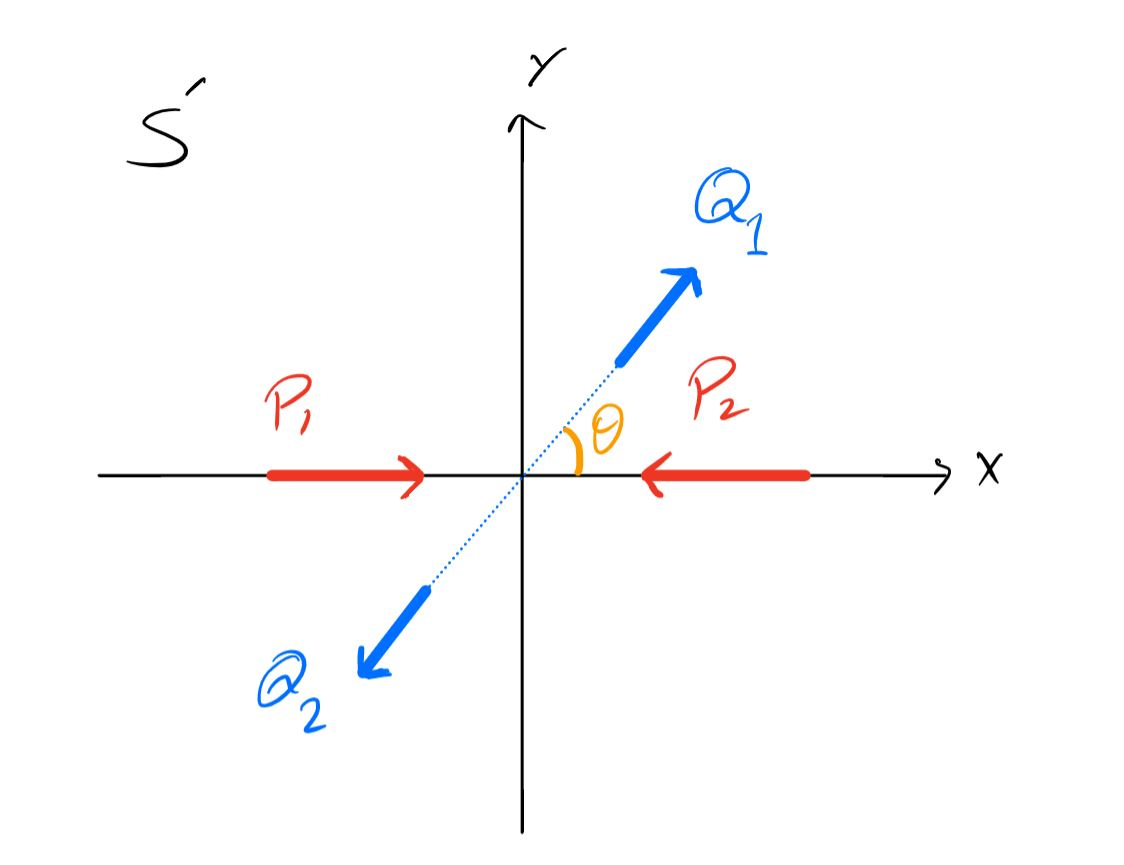
\includegraphics[height=7cm, width=9cm]{4.JPG}
\end{center}

$
  \begin{cases}
    \sum\limits ~ P_{Total}=0 \Longleftrightarrow \overrightarrow{P_1}+\overrightarrow{P_2}=\overrightarrow{Q_1}+\overrightarrow{Q_2}=0
    \\
    \\
    \dfrac{\bigg|\overrightarrow{P_1}\bigg|^2}{2m_1}+\dfrac{\bigg|\overrightarrow{P_2}\bigg|^2}{2m_2}
    =\dfrac{\bigg|\overrightarrow{Q_1}\bigg|^2}{2m_1}+\dfrac{\bigg|\overrightarrow{Q_2}\bigg|^2}{2m_2}
  \end{cases}
  \\
  \\
  \\
  \\
  \therefore ~~~ \dfrac{\bigg|\overrightarrow{P_1}\bigg|^2}{2m_1}+\dfrac{\bigg|\overrightarrow{-P_1}\bigg|^2}{2m_2}
  =\dfrac{\bigg|\overrightarrow{Q_1}\bigg|^2}{2m_1}+\dfrac{\bigg|\overrightarrow{-Q_1}\bigg|^2}{2m_2}
  \Longrightarrow
  \bigg|\overrightarrow{P_1}\bigg|^2 \bigg(\dfrac{1}{2m_1}+\dfrac{1}{2m_2} \bigg)
  =\bigg|\overrightarrow{Q_1}\bigg|^2 \bigg(\dfrac{1}{2m_1}+\dfrac{1}{2m_2} \bigg)
  \\
  \\
  \\
  \therefore ~~~ \boxed{
    \bigg|\overrightarrow{P_1}\bigg|
    =\bigg|\overrightarrow{P_2}\bigg|
    =\bigg|\overrightarrow{Q_1}\bigg|
    =\bigg|\overrightarrow{Q_2}\bigg|
  } ~~~~ \checkmark
$

\begin{center}
  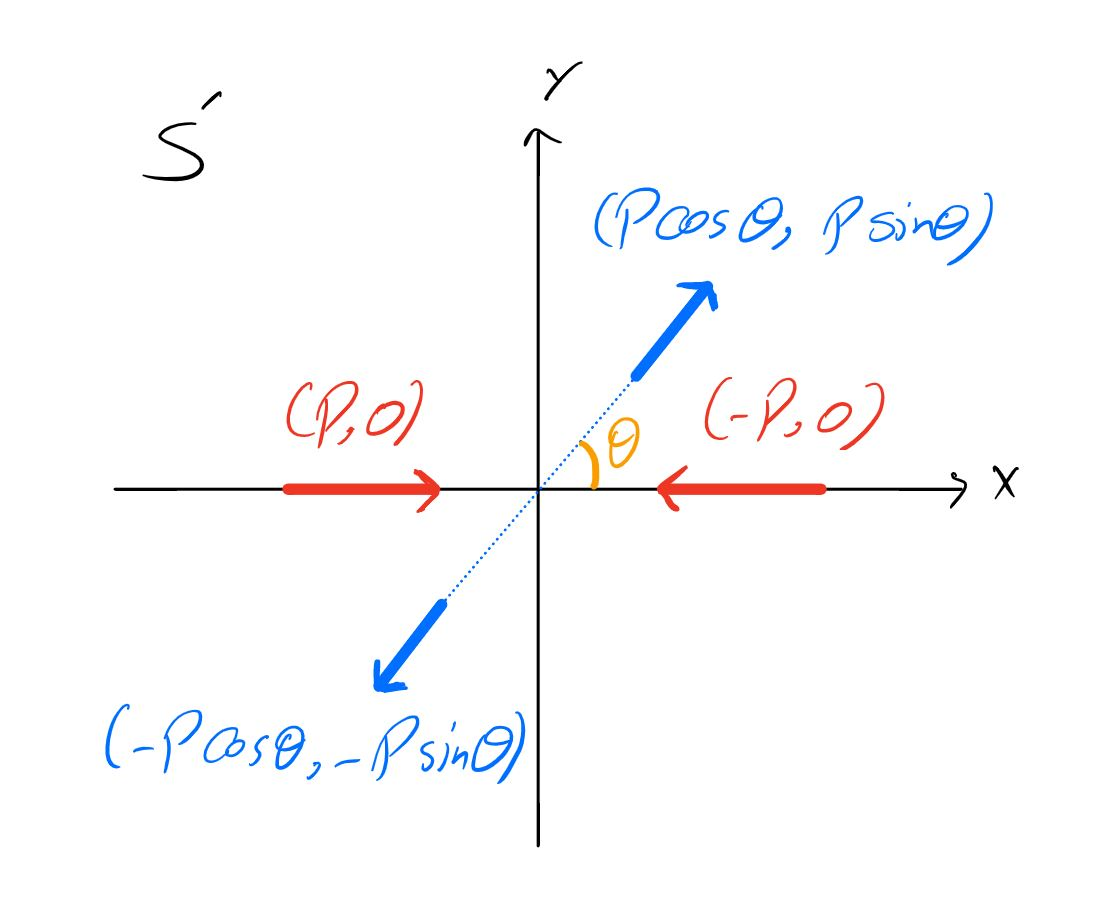
\includegraphics[height=7cm, width=9cm]{5.JPG}
\end{center}

$
  \\
  P=m_1 ~ V_1
  \\
  \\
  V_1=v_1-v_{cm}=v_1-\dfrac{m_1 ~ v_1}{m_1+m_2}
  =\dfrac{v_1 ~ m_1+v_1 ~ m_2-m_1 ~ v_1}{m_1+m_2}
  \\
  \\
  \\
  \therefore ~~~ V_1=\dfrac{v_1 ~ m_2}{m_1+m_2} ~~~~ \checkmark
  \\
  \\
  \\
  \therefore ~~~ P=m_1 \times \dfrac{v_1 ~ m_2}{m_1+m_2}, ~~~~~~ \mu \equiv \dfrac{m_1}{m_1+m_2}
  \\
  \\
  \\
  \therefore ~~~ \boxed{
    P=\mu ~ v_1
  } ~~~~ \checkmark
$

\pagebreak

Velocities in the Center of Mass frame

\begin{center}
  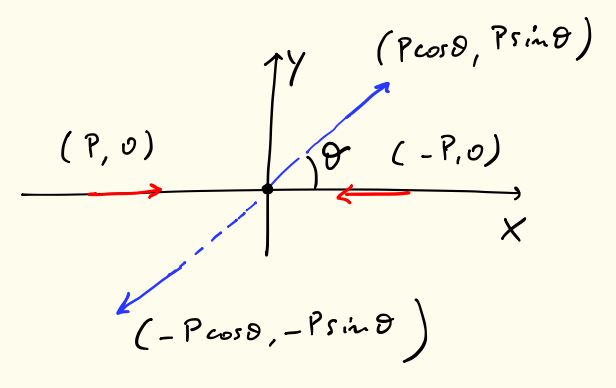
\includegraphics[height=7cm, width=9cm]{6.JPG}
\end{center}

$
  \\
  \begin{cases}
    \overrightarrow{V_1}=\dfrac{1}{m_1} \bigg( P,0 \bigg)
    \\
    \\
    \overrightarrow{V_2}=\dfrac{1}{m_2} \bigg( -P,0 \bigg)
  \end{cases}, ~~~~~~~
  \begin{cases}
    \overrightarrow{U_1}=\dfrac{P}{m_1} \bigg( cos \theta, sin \theta \bigg)
    \\
    \\
    \overrightarrow{U_2}=-\dfrac{P}{m_2} \bigg( cos \theta, sin \theta \bigg)
  \end{cases}
  \\
  \\
$

Convert back to the Lab frame

\vspace{10px}

$
  \\
  \overrightarrow{u_1}=\overrightarrow{U_1}+\overrightarrow{v_{cm}}
  =\dfrac{P}{m_1} \bigg( cos \theta, sin \theta \bigg)+ \bigg( \dfrac{m_1 ~ v_1}{m_1+m_2}, 0\bigg)
  =\dfrac{m_1 ~ m_2 ~ v_1}{m_1+m_2} \dfrac{1}{m_1} \bigg( cos \theta, sin \theta \bigg)
  +\bigg( \dfrac{m_1 ~ v_1}{m_1+m_2}, 0\bigg)
  \\
  \\
  \boxed{\eta \equiv \dfrac{m_1}{m_2} }
  \Longrightarrow \overrightarrow{u_1}=v_1 ~ \left[
    \dfrac{1}{1+\eta} cos \theta+\dfrac{\eta}{\eta+1}, \dfrac{1}{\eta+1} sin \theta
  \right]
  \\
  \\
  \\
  \therefore ~~~ \overrightarrow{u_1}=\dfrac{v_1}{1+\eta} \bigg( cos \theta+\eta, sin \theta \bigg)
  \\
  \\
  \\
  \\
  \\
  \\
  \overrightarrow{u_2}=\overrightarrow{U_2}+\overrightarrow{v_{cm}}
  =-\dfrac{P}{m_2} ~ \bigg( cos \theta, sin \theta \bigg)+ \bigg( \dfrac{m_1 ~ v_1}{m_1+m_2}, 0\bigg)
  \\
  \\
  =-\dfrac{1}{m_2} \dfrac{m_1 ~ m_2}{m_1+m_2} ~ v_1 \bigg( cos \theta, sin \theta \bigg)+ \bigg( \dfrac{m_1 ~ v_1}{m_1+m_2}, 0\bigg)
  =-\dfrac{\eta}{1+\eta} v_1 \bigg( cos \theta, sin \theta \bigg)+\dfrac{\eta}{1+\eta}  \bigg( 1, 0 \bigg)
  \\
  \\
  =\dfrac{\eta}{1+\eta} v_1 \left[
    \bigg( -cos \theta+1, -sin \theta \bigg)
  \right]
  \\
  \\
  \\
  \\
  \therefore ~~~ \boxed{
    \begin{cases}
      \overrightarrow{u_1}=\dfrac{v_1}{1+\eta} \bigg( cos \theta+\eta, sin \theta \bigg)
      \\
      \\
      \overrightarrow{u_2}=\dfrac{v_1}{1+\eta} \bigg( -\eta cos \theta+\eta , -\eta sin \theta \bigg)
    \end{cases}
  } ~~~~ \checkmark
$

\pagebreak

\begin{center}
  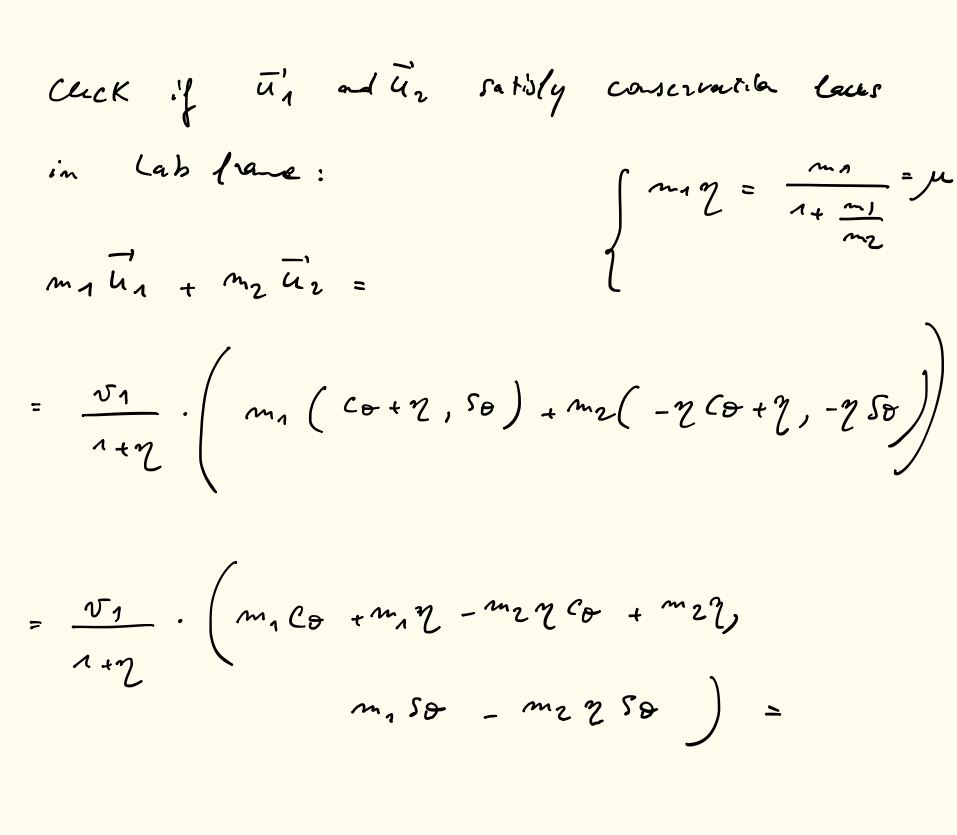
\includegraphics[height=18cm, width=18cm]{7.JPG}
\end{center}

\pagebreak

\begin{center}
  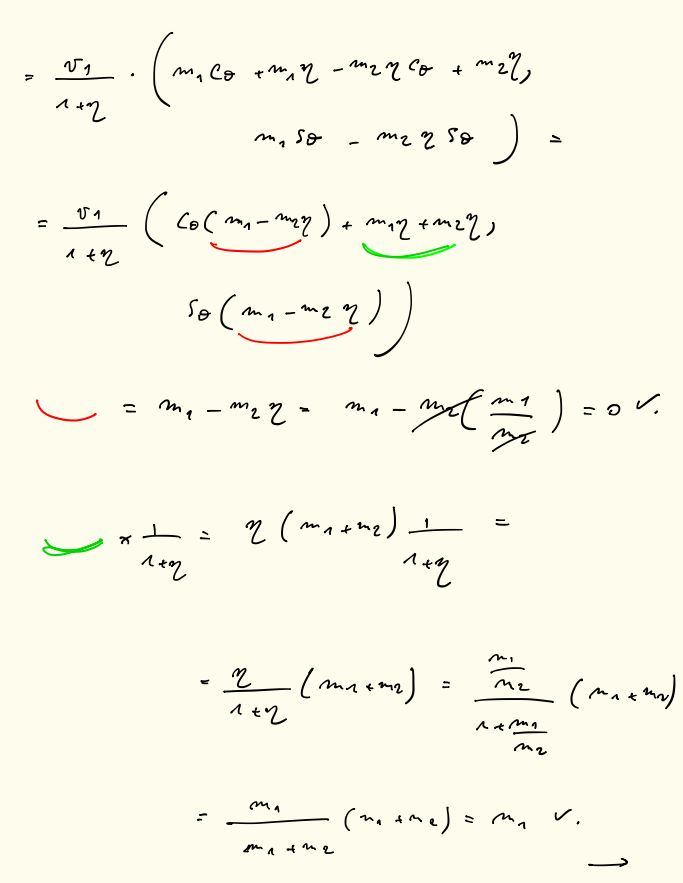
\includegraphics[height=18.5cm, width=18cm]{8.JPG}
\end{center}

\pagebreak

\begin{center}
  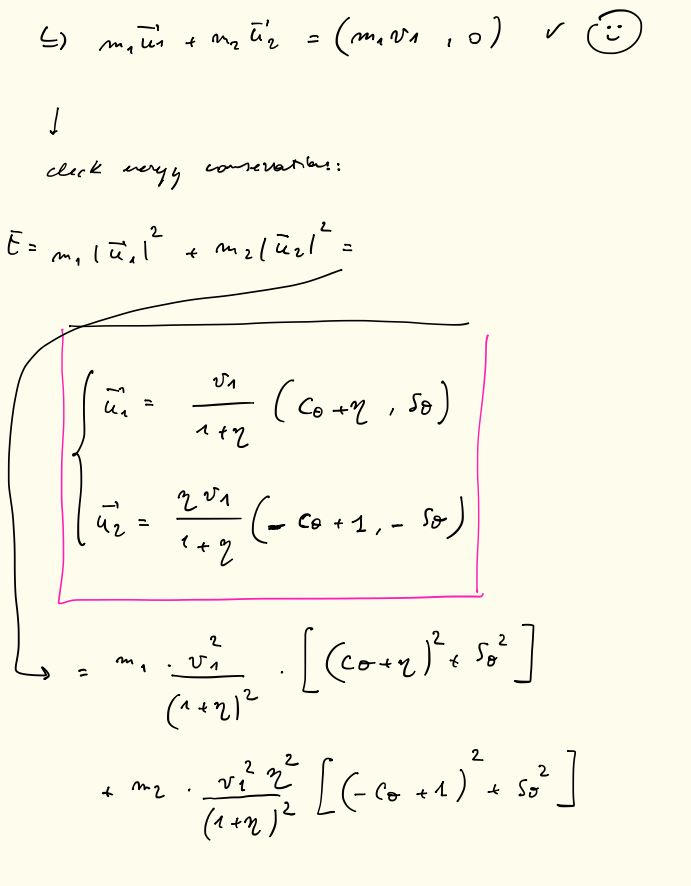
\includegraphics[height=18.5cm, width=18cm]{9.JPG}
\end{center}

\pagebreak

\begin{center}
  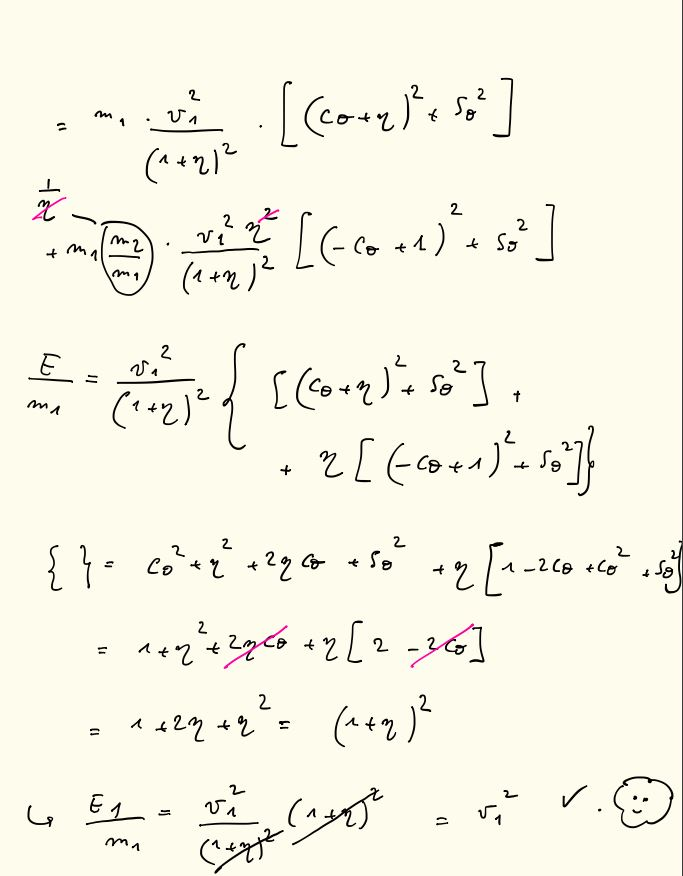
\includegraphics[height=18.5cm, width=18cm]{10.JPG}
\end{center}

\pagebreak

\begin{center}
  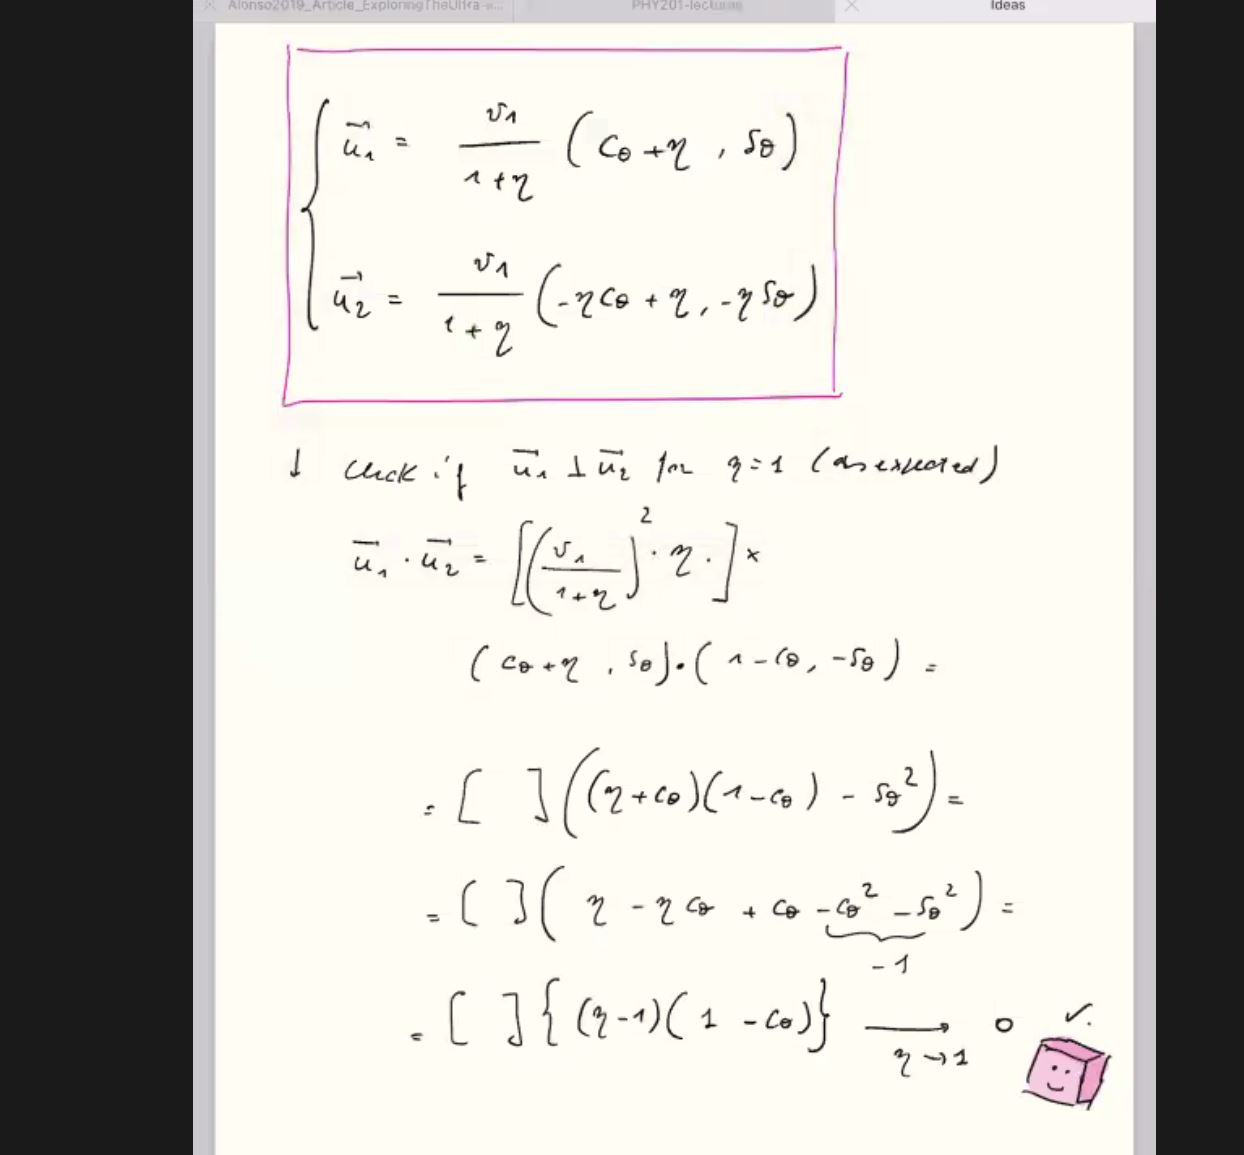
\includegraphics[height=18.5cm, width=18cm]{11.JPG}
\end{center}

\pagebreak

\textbf{Non-head-on relativistic elastic collision of balls in CM frame}

\vspace{10px}

An object's \emph{center of mass} can be thought of as the point where the total mass of an object or a 
system is treated as a point mass. The center of mass of a system of particles is a specific point at 
which the system's mass behaves as if it were concentrated. 

Another way of expressing the \emph{center of mass} is a point where if whole of the mass of the body gets concentrated, 
and then the body is balanced at this point then it experiences no net torque and will remain in static equilibrium.

$$
  x_{cm}=\dfrac{
    \sum\limits_{i=1}^{n} ~ m_i ~ r_i
  }{
    \sum\limits_{i=1}^{n} ~ m_i
  } ~~~~~~~~~~~~
  v_{cm}=\dfrac{
    \sum\limits_{i=1}^{n} ~ p_i
  }{
    \sum\limits_{i=1}^{n} ~ m_i
  }
$$

A quick description of what the laboratory frame and center of mass references are. The \emph{laboratory frame} is a frame 
whereby positions and velocities are measured with respect to the laboratory and the \emph{center of mass} frame is a frame 
whereby the positions and velocities are measured with respect to the the center of mass of a system. Basically, we need 
to change to a moving coordinate system which goes with the velocity of the center of mass.\textbf{ The total momentum 
is always zero in the center of mass reference frame}.

\vspace{20px}

\textbf{Non-Relativistic \& Relativistic}

\vspace{10px}

"Non-relativistic" means based on Newtonian mechanics, whereas “relativistic” means based on the modified theory 
of mechanics included in \textbf{Special Relativity} or the further modified theory included in \textbf{General Relativity}.
In general, non-relativistic limit for a moving particle is to assume that its velocity is much smaller than the 
speed of light, i.e. that
$$
  \dfrac{v}{c} << 1
$$
In this limit, the laws of Special Relativity coincide with the laws of Newtonian physics, and (most) relativistic effects
can be ignored. For example, in Special Relativity the equations that govern the transformations from one inertial frame S 
to another S' that's moving with a velocity $v$ with respect to $S$ are the \textbf{Lorentz Transformations}:
$$
  \begin{cases}
    x^'=\gamma ~ \bigg( x-vt \bigg)
    \\
    \\
    t^'=\gamma ~ \bigg( t-\dfrac{v}{c^2}x \bigg)
  \end{cases}
$$
where 
$$
  \gamma=\dfrac{1}{\sqrt{1-\bigg( \dfrac{v}{c} \bigg)^2}}
$$

The energy of a (massive) particle in Special Relativity is given by:
$$
  E=\gamma ~ mc^2 \approx mc^2+\dfrac{1}{2} mv^2+...
$$
The first term in the expansion above is the rest mass (energy) and the second is the "kinetic" energy. If a 
particle's total kinetic energy is much larger than its rest mass energy, you should be able to see that this 
means the particle is "relativistic".

\vspace{10px}

\textbf{The Energy-Momentum}

\vspace{10px}

The strategy for studying relativistic collisions is the same as that for studying non-relativistic ones. You simply
have to write down all the conservation of energy and momentum equations, and then solve for whatever variables
you want to solve for. The conservation principles are the same as they've always been. It's just that now the
energy and momentum take the new forms $E=\gamma ~ mc^2$ and $\overrightarrow{p}=\gamma ~ m \overrightarrow{v}$.

% \begin{center}
%   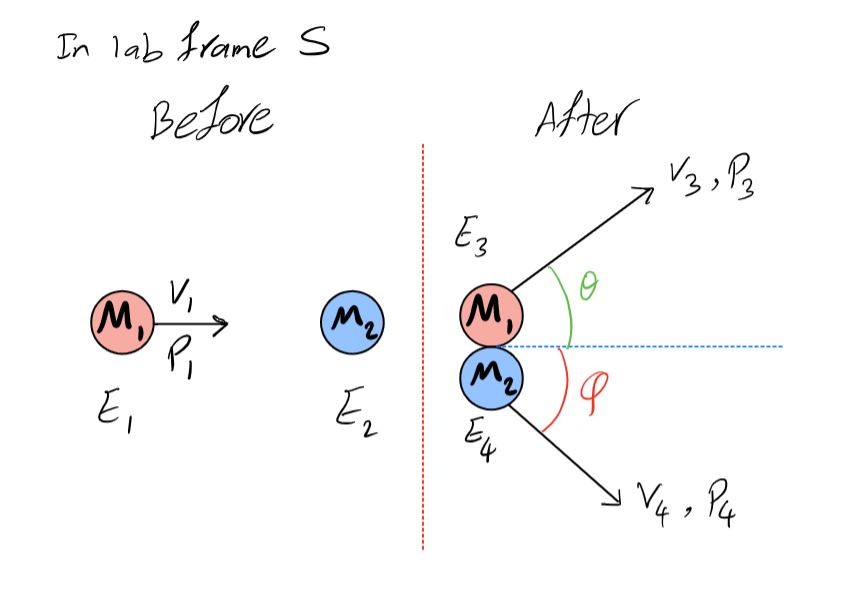
\includegraphics[height=10cm, width=14cm]{12.JPG}
% \end{center}

% \begin{center}
%   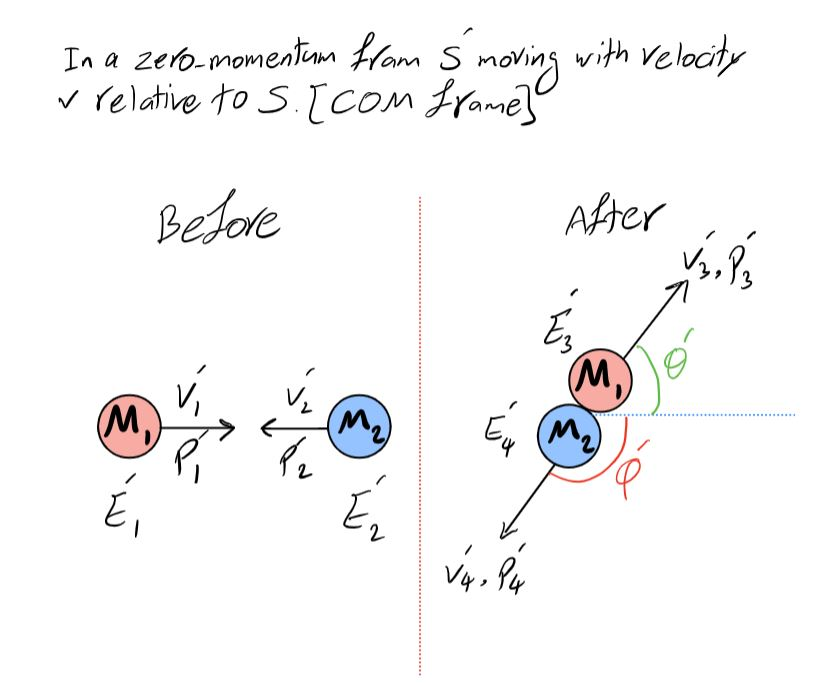
\includegraphics[height=12cm, width=14cm]{13.JPG}
% \end{center}

In center of mass frame

$
  \\
  \begin{cases}
    x_{cm}=\dfrac{
      \sum\limits_{i=1}^{n} ~ m_i ~ r_i
    }{
      \sum\limits_{i=1}^{n} ~ m_i
    }=\dfrac{m_1 ~ x_1+m_2 ~ x_2}{m_1+m_2} ~ \hat{x}
    \\
    \\
    \\
    v_{cm}=\dfrac{
      \sum\limits_{i=1}^{n} ~ p_i
    }{
      \sum\limits_{i=1}^{n} ~ m_i
    }=\dfrac{m_1 ~ v_1+m_2 ~ v_2}{m_1+m_2}=\dfrac{m_1 ~ v_1}{m_1+m_2} ~ \hat{x}
  \end{cases}
  \\
  \\
  \\
$

\textbf{Relativistic Momentum}

\vspace{10px}

Relativistic momentum $\overrightarrow{p}$ is classical momentum multiplied by the relativistic factor 
$\gamma$, so it is $\overrightarrow{p}=\gamma ~ m \overrightarrow{v}=\dfrac{m \overrightarrow{v}}{\sqrt{1-\dfrac{v^2}{c^2}}}$
where p denotes momentum of any particle with mass, v denotes velocity, and c is the speed of light.

\vspace{20px}

\textbf{Relativistic Energy}

\vspace{10px}

$
  W=KE=\bigints F.ds=\bigints \dfrac{d}{dt} \bigg( \gamma m v \bigg) ~ ds, ~~~ ds=v ~ dt
  \\
  \\
  \\
  KE=\bigints \dfrac{d}{dt} \bigg( \gamma m v \bigg) ~ v dt=m \bigints dt \dfrac{d}{dt} \bigg( \gamma v \bigg) v
  =\bigints\limits_{0}^{ \gamma V} ~ v d\bigg( \gamma v\bigg)
  =\gamma m V^2-m \bigints\limits_{0}^{V} \gamma v dv
  \\
  \\
  \\
  =\gamma m V^2-m \bigints\limits_{0}^{V}  \dfrac{v dv}{\sqrt{1-\dfrac{v^2}{c^2}}}
  =\gamma m V^2+mc^2 \sqrt{1-\dfrac{v^2}{c^2}} \Big|_{0}^{V}
  \\
  \\
  \\
  \therefore ~~~ \boxed{
    KE=mc^2~ \bigg( \gamma -1 \bigg)
  } ~~~~ \checkmark
  \\
  \\
$

This expression does not look the kinetic energy formula in non-relativistic which is $\dfrac{1}{2} mv^2$, but when dealing 
with really small velocities than the speed of light. 

$
  \\
  \\
  \gamma=\dfrac{1}{\sqrt{1-\dfrac{v^2}{c^2}}}=\bigg( 1-\dfrac{v^2}{c^2} \bigg)^{-1/2} \approx 1+\dfrac{1}{2} \dfrac{v^2}{c^2}+...
  \\
  \\
  \\
  \longrightarrow KE=mc^2~ \bigg( \gamma -1 \bigg) \approx \dfrac{1}{2} \dfrac{v^2}{c^2} mc^2
  \\
  \\
  \\
  \therefore ~~~ \boxed{
    KE=\dfrac{1}{2} mv^2, ~~~~ v << c 
  } ~~~~ \checkmark
  \\
  \\
  \\
$

\textbf{Relationship between Energy and Momentum}

\vspace{10px}

In the Newtonian, we have $E=\dfrac{1}{2} ~ mv^2$ and $p=mv$, therefore $\boxed{E=\dfrac{p^2}{2m}}$. In the relativistic case though
we have the following definitions:

$
  \\
  \\
  \begin{cases}
    E=\gamma ~ mc^2
    \\
    \\
    p=\gamma ~ mv
    \\
    \\
    \gamma=\dfrac{1}{\sqrt{1-\dfrac{v^2}{c^2}}}
  \end{cases} \Longrightarrow p^2 ~ c^2=\gamma^2 ~ m^2 ~ v^2 ~ c^2=\gamma^2 ~ m^2 ~ c^4 ~ \dfrac{v^2}{c^2}
  =\gamma^2 ~ m^2 ~ c^4 \bigg( 1-\dfrac{1}{\gamma^2} \bigg)
  \\
  \\
  \\
  p^2 ~ c^2=\gamma^2 ~ m^2 ~ c^4 - m^2 ~ c^4
  \\
  \\
  \\
  \therefore ~~~ \boxed{
    E^2=p^2 ~ c^2+m^2 ~ c^4
  } ~~~~~~ (I)
  \\
  \\
  \\
$

The equations for momentum conservation remain the same as non-relativistic case, so we have:

$
  \\
  \\
  \text{Momentum x-direction} ~~~ (I): ~~~ P_0+0=P_2 ~ cos\theta+P_3 ~ cos \phi
  \\
  \\
  \text{Momentum y-direction} ~~~ (II): ~~~ 0=P_2 ~ sin\theta -P_3 ~ sin \phi
  \\
  \\
 $

Before the collision occurs, one particle is moving and the one other is stationary. As the result of this 
configuration, the energy of the first particle is $E_0$ and the rest-mass energy of the stationary particle 
is $m_1 c^2$. \emph{The rest-mass energy is the energy that is stored inside a stationary particle as a result of its mass}.
Rest-mass energy implies that mass is simply another form of energy. In fact, experiments readily show that mass 
can be converted to energy (nuclear decay) and energy can be converted to mass (photon-pair production). Hence, we have:

$
  \\
  E_0+m_1 c^2=E_2+E_3=E_{tot} \Longrightarrow \boxed{E_3=E_{tot}-E_2} ~~~~~~ (II)
  \\
  \\
  \begin{cases}
    P_0-P_2 cos \theta=P_3 cos \phi
    \\
    \\
    P_2 sin \theta=-P_3 sin \phi
  \end{cases}
  \\
  \\
$

Squaring and adding the above gives

$
  \\
  \begin{cases}
    P^2_0+P^2_2 ~ cos^2\theta-2P_0 P_2 ~ cos \theta=P^2_3 ~ cos^2 \phi
    \\
    \\
    P^2_2 ~ sin^2\theta=P^2_3 ~ sin^2 \phi
  \end{cases} 
  \\
  \\
  \\
  P^2_0+P^2_2 ~ cos^2\theta-2P_0 P_2 ~ cos \theta+P^2_2 ~ sin^2\theta=P^2_3 ~ cos^2 \phi+P^2_3 ~ sin^2 \phi
  \\
  \\
  P^2_0+P^2_2 \bigg( cos^2\theta+sin^2\theta \bigg)-2P_0 P_2 ~ cos \theta=P^2_3 \bigg( cos^2 \phi+sin^2 \phi \bigg)
  \\
  \\
  P^2_0+P^2_2-2P_0 P_2 ~ cos \theta=P^2_3
  \\
$

Multiplying both sides by $c^2$ gives $P^2_0 ~ c^2 +P^2_2 ~ c^2 -2P_0 P_2 c^2 ~ cos \theta=P^2_3 ~ c^2 ~~ (III)$. From equation $(I)$ we know
$P^2 c^2=E^2-\bigg( m c^2 \bigg)^2$ , hence we rewrite the $R.H.S$ of $(III)$ with the help of $(II)$ as:

$
  \\
  P^2_0 ~ c^2 +P^2_2 ~ c^2 -2P_0 P_2 c^2 ~ cos \theta=P^2_3 ~ c^2=E^2_3-\bigg( m_3 c^2 \bigg)^2=\bigg( E_{tot}-E_2 \bigg)^2-\bigg( m_3 c^2 \bigg)^2
  \\
  \\
  \\
  P^2_0 ~ c^2 +P^2_2 ~ c^2 -2P_0 P_2 c^2 ~ cos \theta=E^2_{tot}+E^2_2-2 E_{tot} E_2-m^2_3 c^4
  \\
  \\
  \\
  P^2_0 ~ c^2 +\bigg( P^2_2 ~ c^2 \bigg) -2P_0 P_2 c^2 ~ cos \theta=E^2_{tot}+E^2_2-2 E_{tot} E_2-m^2_3 c^4
  \\
  \\
  \\
  P^2_0 ~ c^2 +\bigg( E^2_2-m^2_2 c^4 \bigg) -2P_0 P_2 c^2 ~ cos \theta=E^2_{tot}+E^2_2-2 E_{tot} E_2-m^2_3 c^4
  \\
  \\
  \\
  P^2_0 ~ c^2+E^2_2-m^2_2 c^4-2 P_0 P_2 c^2 cos \theta-E^2_2+m^2_3 c^4=E^2_{tot}-2E_{tot} E_2
  \\
  \\
  \\
  2 P_0 P_2 c^2 cos\theta=P^2_0 c^2-m^2_2 c^4+m^2_3 c^4-E^2_{tot}+2 E_{tot} E_2
  \\
$

Squaring both sides of the above leads to

$
  \\
  4 P^2_0 P^2_2 c^4 cos^2\theta=\bigg( m^2_3 c^4-m^2_2 c^4+P_0^2 c^2+2 E_{tot} E_2-E^2_{tot} \bigg)^2
  \\
  \\
  \\
  \text{Note:} ~~ \boxed{
    \bigg( a+b+c+d+e \bigg)^2=a^2+b^2+c^2+d^2+e^2+2ac+2ad-2ab-2ae+2be-2bc-2ce-2bd+2cd-2de
  }
  \\
  \\
  \\
  R.H.S: ~~~ \left[
    m^2_3 c^4-m^2_2 c^4+P_0^2 c^2+2 E_{tot} E_2-E^2_{tot}
  \right]^2
  \\
  \\
  =m^4_3 c^8-m^4_2 c^8+P^4_0 c^4+4 E^2_{tot} E^2_2-E^4_{tot}
  +2m^2_3 c^4 P^2_0 c^2
  +4 m^2_3 c^4 E_{tot} E_2
  -2 m^2_3 c^8 m^2_2
  -2m^2_3 c^4 E^2_{tot}
  +2 m^2_2 c^4 E^2_{tot}
  -2 m^2_2 c^4 P^2_0 c^2
  -2P^2_0 c^2 E^2_{tot}
  -4 m^2_2 c^4 E_{tot} E_2
  +4 P^2_0 c^2 E_{tot} E_2-4E^3_{tot} E_2
  \\
  \\
  \\
  \\
  \therefore ~~~ 4 P^2_0 \bigg( E^2_2-m^2_2 c^4 \bigg) c^2 cos^2 \theta
  =m^4_3 c^8-m^4_2 c^8+P^4_0 c^4+4 E^2_{tot} E^2_2-E^4_{tot}
  +2m^2_3 c^4 P^2_0 c^2
  +4 m^2_3 c^4 E_{tot} E_2
  -2 m^2_3 c^8 m^2_2
  -2m^2_3 c^4 E^2_{tot}
  +2 m^2_2 c^4 E^2_{tot}
  -2 m^2_2 c^4 P^2_0 c^2
  -2P^2_0 c^2 E^2_{tot}
  -4 m^2_2 c^4 E_{tot} E_2
  +4 P^2_0 c^2 E_{tot} E_2-4E^3_{tot} E_2
  \\
  \\
  \\
  \\
  4 P^2_0 ~ E^2_2 ~ c^2 cos^2 \theta-4 P^2_0 ~ c^2 cos^2 \theta m^2_2 c^4
  =m^4_3 c^8-m^4_2 c^8+P^4_0 c^4+4 E^2_{tot} E^2_2-E^4_{tot}
  +2m^2_3 c^4 P^2_0 c^2
  +4 m^2_3 c^4 E_{tot} E_2
  -2 m^2_3 c^8 m^2_2
  -2m^2_3 c^4 E^2_{tot}
  +2 m^2_2 c^4 E^2_{tot}
  -2 m^2_2 c^4 P^2_0 c^2
  -2P^2_0 c^2 E^2_{tot}
  -4 m^2_2 c^4 E_{tot} E_2
  +4 P^2_0 c^2 E_{tot} E_2-4E^3_{tot} E_2
  \\
  \\
  \\
  \\
  E^2_2 \bigg( 4 P^2_0 c^2 cos^2 \theta -4 E^2_{tot} \bigg)
  +E_2 \bigg( 4 E^3_{tot}-4 P^2_0 c^2 E_{tot}+4 m^2_2 c^4 E_{tot}-4m^2_3 c^4 E_{tot} \bigg)
  +\bigg(
    -4 m^2_2 c^4 P^2_0 c^2 cos^2 \theta
    +2 m^2_3 c^4 m^2_2
    +2 P^2_0 c^2 E^2_{tot}
    -2 m^2_2 c^4 E^2_{tot}
    +2 P^2_0 m^2_2 c^6
    +2 m^2_3 c^4 E^2_{tot}
    -2 P^2_0 m^2_3 c^6
    -E^4_{tot}-P^4_0 c^4 
    -m^4_2 c^8 
    -m^4_3 c^8
  \bigg)
  =0 ~~~~~~ (IV)
  \\
  \\
$

Now it is time to solve this quadratic equation for $E_2=\dfrac{-b \pm \sqrt{b^2-4ac}}{2a}$. By knowing $E_2$ we can calculate the following items:

$
  \\
  \\
  \therefore ~~~ \boxed{
    \begin{cases}
      KE_2=E_2-m_2 c^2
      \\
      \\
      E_3=E_{tot}-E_2
      \\
      \\
      KE_3=E_3-m_3 c^2
      \\
      \\
      P_2=\sqrt{E^2_2-m^2_2 c^4}
      \\
      \\
      P_3=\sqrt{E^2_3-m^2_3 c^4}
      \\
      \\
      \phi=sin^{-1} \bigg( \dfrac{P_2}{P_3}  sin \theta \bigg)
    \end{cases}
  } ~~~~ \checkmark
  \\
  \\
$

% The system we are working on has two particles in it. Let's name particles $0$ and $2$ which are the same 
% particles but we used different numbers to indicate the before and after state of the collision, particle $a$ and let's
% rename particle $1$ and $3$ which again are the same particle $b$. Also, 
For simplicity, we assume $c=1$ therefore equation $(IV)$ becomes 

$
  \\
  E^2_2 \bigg( 4 P^2_0 cos^2 \theta -4 E^2_{tot} \bigg)
  +E_2 \bigg( 4 E^3_{tot}-4 P^2_0 E_{tot}+4 m^2_2 E_{tot}-4m^2_3 E_{tot} \bigg)
  +\bigg(
    -4 m^2_2 P^2_0 cos^2 \theta
    +2 m^2_3 m^2_2
    +2 P^2_0 E^2_{tot}
    -2 m^2_2 E^2_{tot}
    +2 P^2_0 m^2_2
    +2 m^2_3 E^2_{tot}
    -2 P^2_0 m^2_3
    -E^4_{tot}-P^4_0 
    -m^4_2 
    -m^4_3
  \bigg)
  =0
  \\
  \\
  \\
  \Longrightarrow \begin{cases}
    a=\bigg( 4 P^2_0 cos^2 \theta -4 E^2_{tot} \bigg)
    \\
    \\
    b=\bigg( 4 E^3_{tot}-4 P^2_0 E_{tot}+4 m^2_2 E_{tot}-4m^2_3 E_{tot} \bigg)
    \\
    \\
    c=\bigg(
      -4 m^2_2 P^2_0 cos^2 \theta
      +2 m^2_3 m^2_2
      +2 P^2_0 E^2_{tot}
      -2 m^2_2 E^2_{tot}
      +2 P^2_0 m^2_2
      +2 m^2_3 E^2_{tot}
      -2 P^2_0 m^2_3
      -E^4_{tot}-P^4_0 
      -m^4_2 
      -m^4_3
    \bigg)
  \end{cases}
  \\
  \\
  \\
  E_2=\dfrac{-b \pm \sqrt{b^2-4ac}}{2a}
$

\pagebreak

\textbf{Relativistic kinematics in the COM frame}

\vspace{10px}

The COM velocity in the initial frame is

$
  \\
  \\
  v^i_{cm}=\dfrac{P_0+P_1}{E_0+E_1}=\dfrac{P_0}{E_{tot}}
  \\
  \\
$

From the conservation of momentum in the initial and final frames:

$
  \\
  \\
  \gamma^i_{cm} \bigg( m_0+m_1\bigg) \dfrac{v^i_{cm}}{c}=\gamma^f_{cm} \bigg( m_2+m_3\bigg) \dfrac{v^f_{cm}}{c}
  \\
  \\
  \\
  \gamma^i_{cm} \dfrac{m_0+m_1}{m_2+m_3} \dfrac{v^i_{cm}}{c}=\dfrac{v^f_{cm}/c}{\sqrt{1-\bigg( \dfrac{v^f_{cm}}{c}\bigg)^2}}
  \\
  \\
  \\
  \bigg( \gamma^i_{cm} \dfrac{m_0+m_1}{m_2+m_3} \dfrac{v^i_{cm}}{c} \bigg)^2=\bigg( \dfrac{v^f_{cm}/c}{\sqrt{1-\bigg( \dfrac{v^f_{cm}}{c}\bigg)^2}} \bigg)^2
  \\
  \\
  \\
  \bigg( \gamma^i_{cm} \dfrac{m_0+m_1}{m_2+m_3} \dfrac{v^i_{cm}}{c} \bigg)^2=\dfrac{\bigg( v^f_{cm}/c \bigg)^2}{1-\bigg( \dfrac{v^f_{cm}}{c}\bigg)^2}
  \\
  \\
  \\
  \bigg( v^f_{cm}/c \bigg)^2=\dfrac{
    \bigg( \gamma^i_{cm} \dfrac{m_0+m_1}{m_2+m_3} \dfrac{v^i_{cm}}{c} \bigg)
  }{
    1+\bigg( \gamma^i_{cm} \dfrac{m_0+m_1}{m_2+m_3} \dfrac{v^i_{cm}}{c} \bigg)
  }
  \\
  \\
  \\
  \therefore ~~~ \boxed{
    \dfrac{v^f_{cm}}{c}=\dfrac{
      \bigg( \gamma^i_{cm} \dfrac{m_0+m_1}{m_2+m_3} \dfrac{v^i_{cm}}{c} \bigg)
    }{
      1+\bigg( \gamma^i_{cm} \dfrac{m_0+m_1}{m_2+m_3} \dfrac{v^i_{cm}}{c} \bigg)
    }
  } ~~~~ \checkmark
  \\
  \\
$

The COM total and kinetic energies are calculated as

$
  \\
  \\
  \boxed{
    \begin{cases}
      E_{cm0}=\gamma^i_{cm} \bigg( E_0- c P_0 v^i_{cm} \bigg)
      \\
      \\
      E_{cm1}=\gamma^i_{cm} \bigg( E_1- c P_1 v^i_{cm} \bigg)
    \end{cases}, ~~~~~ 
    \begin{cases}
      KE_{cm0}=E_{cm0}-m_0 c^2
      \\
      \\
      KE_{cm1}=E_{cm1}-m_1 c^2
    \end{cases}
  } ~~~~ \checkmark
  \\
  \\
$

Using Lorentz's transformation matrix for ball 0 we have:

$
  \\
  \\
  \begin{pmatrix}
    P_{cm0} c
    \\
    0
    \\
    0
    \\
    \dfrac{E_{cm0}}{c}
  \end{pmatrix}=
  \begin{pmatrix}
    \gamma^i_{cm} && 0 && 0 && -\gamma^i_{cm} \dfrac{v^i_{cm}}{c}
    \\
    0 && 1 && 0 && 0
    \\
    0 && 0 && 1 && 0
    \\
    -\gamma^i_{cm} \dfrac{v^i_{cm}}{c} && 0 && 0 && \gamma^i_{cm}
  \end{pmatrix}
  \begin{pmatrix}
    P_0 c
    \\
    0
    \\
    0
    \\
    \dfrac{E_0}{c}
  \end{pmatrix}
  \\
  \\
$

Similar for the outgoing (final) frame balls 2 and 3 (after collision)

$
  \\
  \\
  \begin{pmatrix}
    P_{cm3} c cos \phi_{cm}
    \\
    P_{cm3} c sin \phi_{cm}
    \\
    0
    \\
    \dfrac{E_{cm3}}{c}
  \end{pmatrix}=
  \begin{pmatrix}
    \gamma^i_{cm} && 0 && 0 && -\gamma^i_{cm} \dfrac{v^i_{cm}}{c}
    \\
    0 && 1 && 0 && 0
    \\
    0 && 0 && 1 && 0
    \\
    -\gamma^i_{cm} \dfrac{v^i_{cm}}{c} && 0 && 0 && \gamma^i_{cm}
  \end{pmatrix}
  \begin{pmatrix}
    P_{cm3} ~ c ~ cos \phi
    \\
    P_{cm3} ~ c ~ sin \phi
    \\
    0
    \\
    \dfrac{E_3}{c}
  \end{pmatrix} ~~~~~~~ (A)
  \\
  \\
  \\
  \therefore ~~~ \boxed{
    \begin{cases}
      E_{cm2}=\gamma^f \bigg( E_2-P_2 v^f_{cm} cos \theta  \bigg)
      \\
      \\
      E_{cm3}=\gamma^f \bigg( E_3-P_3 v^f_{cm} cos \theta  \bigg)
    \end{cases}, ~~~~
    \begin{cases}
      KE_{cm2}=E_{cm2}-m_2 c^2
      \\
      \\
      KE_{cm3}=E_{cm3}-m_3 c^2
    \end{cases}
  } ~~~~ \checkmark
  \\
  \\
$

For relativistic velocities we have

$
  \\
  \\
  v_{cm0}=\dfrac{v_0-v^i_{cm}}{1-\dfrac{v_0 v^i_{cm}}{c^2}} \Longrightarrow v_{cm2} cos \theta_{cm}=\dfrac{v_2 cos \theta - v^i_{cm}}{1-\dfrac{v_0 cos \theta v^i_{cm}}{c^2}}
  \\
  \\
  \\
  \therefore ~~~ v_{cm2} sin \theta_{cm}=v_2 sin \theta
  \\
  \\
  \\
  \text{Knowing that} ~ \dfrac{v}{c}=\dfrac{P c}{E} \Longrightarrow \dfrac{v_{cm}}{c}=\sqrt{1-\dfrac{m^2 c^4}{E^2_{cm}}}
  \\
  \\
  \\
  \dfrac{v_{cm}}{c}=\sqrt{\bigg( \dfrac{P c}{E}\bigg)^2}=\sqrt{\dfrac{E^2-m^2 c^4}{E^2}}
  \\
  \\
  \\
  \therefore ~~~ \boxed{\dfrac{v_{cm}}{c}=\sqrt{1-\bigg( \dfrac{m^2 c^4}{E}\bigg)^2}} ~~~~ \checkmark
  \\
  \\
  \\
  \\
  \\
  \text{From (A) we have }
  \\
  \\
  \\
  \therefore ~~~ \boxed{
    \begin{cases}
      \theta_{cm}=tan^{-1} \bigg( \dfrac{P_2 ~ c ~ sin\theta }{\gamma^f_{cm}  \bigg( P_2 ~ c ~ cos\theta -\dfrac{v^f_{cm}}{c} E_2 \bigg)   } \bigg)
      \\
      \\
      \phi_{cm}=\pi-\theta_{cm}
    \end{cases}
  } ~~~~ \checkmark
  \\
  \\
$

\pagebreak

\textbf{Deriving non-relativistic from relativistic in the COM frame}

\vspace{10px}

When studying the relativistic case we had

\vspace{10px}

$
  \begin{cases}
    \gamma=\dfrac{1}{\sqrt{1-\bigg( \dfrac{v}{c} \bigg)^2}}
    \\
    \\
    p=\gamma ~ m v
    \\
    \\
    E=\gamma ~ m c^2
  \end{cases} \Longrightarrow E=\gamma ~ \dfrac{p}{\gamma v} c^2=\dfrac{pc^2}{v}
  \Longrightarrow \boxed{\dfrac{pc}{E}=\dfrac{v}{c}}
  \\
  \\
$

Let's find an approximation of the Lorentz Factor using the \textbf{Taylor Expansion}:

\vspace{10px}

$
  \\
  \beta \equiv \dfrac{v}{c}
  \Longrightarrow 
  \gamma(\beta)=\dfrac{1}{\sqrt{1-\beta^2}}=\bigg( 1-\beta^2 \bigg)^{-\dfrac{1}{2}}
  \\
  \\
  \\
  \text{Recall that:} 
  \\
  \\
  f(x)=\sum\limits_{n=0}^{\infty} \dfrac{f^n(x_0)}{n!} \bigg( x-x_0 \bigg)^n
  =f(x_0)+\dfrac{f^'(x_0)}{1!} \bigg( x-x_0 \bigg)+\dfrac{f^{''}(x_0)}{2!} \bigg( x-x_0 \bigg)^2+\dfrac{f^{'''}(x_0)}{3!} \bigg( x-x_0 \bigg)^3+...
  \\
  \\
  \\
  \begin{cases}
    \dfrac{d \gamma(\beta)}{d \beta}=\dfrac{d}{d\beta} \left[\bigg( 1-\beta^2 \bigg)^{-\dfrac{1}{2}} \right]
    =\beta \bigg( 1- \beta^2 \bigg)^{-\dfrac{3}{2}}
    \\
    \\
    \\
    \dfrac{d^2 \gamma(\beta)}{d \beta^2}=\dfrac{d \beta}{d \beta} \bigg( 1- \beta^2 \bigg)^{-\dfrac{3}{2}}+\beta \dfrac{d}{d\beta} \bigg( 1- \beta^2 \bigg)^{-\dfrac{3}{2}}
    =\bigg( 1-\beta^2 \bigg)^{-\dfrac{3}{2}}+3 \beta^2 \bigg( 1-\beta^2 \bigg)^{-\dfrac{5}{2}}
  \end{cases}
  \\
  \\
  \\
  \gamma(0)=\gamma(0)+\dfrac{\gamma^'(0)}{1!} \beta+\dfrac{\gamma^{''}(0)}{2!} \beta^2+...
  =1+0+\dfrac{\beta^2}{2}+...
  \\
  \\
  \\
  \therefore ~~~ \boxed{
    \gamma=\dfrac{1}{\sqrt{1-\beta^2}}=\sum\limits_{n=0}^{\infty} \dfrac{\bigg( 2n \bigg)!}{\bigg( 2^n ~ n!\bigg)^2} \beta^{2n}
  } ~~~~ \checkmark
  , ~~~~~~~~~ \therefore ~~~ \boxed{
    \gamma=1+\dfrac{1}{2} \beta^2+\dfrac{3}{8} \beta^4+\dfrac{5}{16} \beta^6+...
  } ~~~~ \checkmark
$

\pagebreak

Generally speaking, non-relativistic limit for a moving particle is to assume that its velocity is much smaller 
than the speed of light, $\dfrac{v}{c} << 1$. Momentum conservation before and after the collision. Considering
the relativistic formula of momentum we have:

\vspace{10px}

$
  \\
  p_0+p_1=p_2+p_3
  \\
  \\
  \\
  \gamma_{cmi} ~ \bigg( m_0+m_1 \bigg)v_{cmi}=\gamma_{cmf} ~ \bigg( m_2+m_3 \bigg) v_{cmf}
  \\
  \\
  \\
  \text{Taking the first two terms of the Lorentz Factor gives us } \gamma=1+\dfrac{1}{2} \dfrac{v^2}{c^2}
  \\
  \\
  \\
  \bigg( 1+\dfrac{1}{2} \dfrac{v^2_{cmi}}{c^2} \bigg) ~ \bigg( m_0+m_1 \bigg)v_{cmi}=\bigg( 1+\dfrac{1}{2} \dfrac{v^2_{cmf}}{c^2} \bigg) ~ \bigg( m_2+m_3 \bigg) v_{cmf}
  \\
  \\
  \\
  v_{cmi} \bigg( 1+\dfrac{1}{2} \dfrac{v^2_{cmi}}{c^2} \bigg) ~ \dfrac{m_0+m_1}{m_2+m_3}=v_{cmf} \bigg( 1+\dfrac{1}{2} \dfrac{v^2_{cmf}}{c^2} \bigg)
  \\
  \\
  \\
  \bigg( v_{cmi}+\dfrac{v^3_{cmi}}{2c^2} \bigg) ~ \dfrac{m_0+m_1}{m_2+m_3}=v_{cmf}+\dfrac{v^3_{cmf}}{2c^2}
  \\
  \\
  \\
  \begin{cases}
    \mathcal{S} \equiv\bigg( v_{cmi}+\dfrac{v^3_{cmi}}{2c^2} \bigg) ~ \dfrac{m_0+m_1}{m_2+m_3}
    \\
    \\
    \mathcal{X} \equiv v_{cmf} 
  \end{cases}
  \Longrightarrow \mathcal{X}+\dfrac{\mathcal{X}^3}{2c^2}=\mathcal{S}
  \\
  \\
  \\
  \mathcal{X}^3+2c^2 \mathcal{X}-2c^2\mathcal{S}=0
  \\
  \\
$

Recall that the general solution to the cubic equation $x^3+px+q=0$ is

$
  \\
  x=\sqrt[3]{-\dfrac{q}{2}-\sqrt{(\dfrac{q}{2})^2+(\dfrac{p}{3})^3}}
  +\sqrt[3]{-\dfrac{q}{2}+\sqrt{(\dfrac{q}{2})^2+(\dfrac{p}{3})^3}}
  \\
  \\
$

It is very important to know that how many solutions our cubic equation has. For positive $p$, 
there can be only one solution, but for a negative $p$, one, two or three solutions are possible. 
To figure out how many solutions we get for negative $p$, we need to determine the difference in height 
between the inflection point and the two extrema.

\pagebreak

$
  \begin{cases}
    p=2c^2
    \\
    \\
    q=-\mathcal{S}
  \end{cases}
  \\
  \\
  \\
  \mathcal{X}=\sqrt[3]{\dfrac{\mathcal{S}}{2}-\sqrt{(\dfrac{\mathcal{S}}{2})^2+(\dfrac{2c^2}{3})^3}}
  +\sqrt[3]{\dfrac{\mathcal{S}}{2}+\sqrt{(\dfrac{\mathcal{S}}{2})^2+(\dfrac{2c^2}{3})^3}}
  \\
  \\
  \\
  =\sqrt[3]{\dfrac{\mathcal{S}}{2}-\sqrt{\dfrac{\mathcal{S}^2}{4}+\dfrac{8c^6}{27}}}
  +\sqrt[3]{\dfrac{\mathcal{S}}{2}+\sqrt{\dfrac{\mathcal{S}^2}{4}+\dfrac{8c^6}{27}}}
  \\
  \\
  \\
$

\pagebreak

$
  \therefore ~~~ \boxed{
    v_{cmf}= v_{cmi} \dfrac{m_0+m_1}{m_2+m_3}
  } ~~~~ \checkmark
  \\
  \\
  \\
  \\
  \gamma_{cmi} ~ \bigg( m_0+m_1 \bigg)v_{cmi} \times \dfrac{1}{c}=\gamma_{cmf} ~ \bigg( m_2+m_3 \bigg) v_{cmf} \times \dfrac{1}{c}
  \\
  \\
  \\
  \dfrac{\gamma_{cmi}}{c} \dfrac{\bigg( m_0+m_1 \bigg)}{\bigg( m_2+m_3 \bigg)} v_{cmi}=\dfrac{v_{cmf}}{c} \dfrac{1}{\sqrt{1-\bigg( \dfrac{v_{cmf}}{c} \bigg)^2}}
  \\
  \\
  \\
  \left[ \dfrac{\gamma_{cmi}}{c} \dfrac{\bigg( m_0+m_1 \bigg)}{\bigg( m_2+m_3 \bigg)} v_{cmi} \right]^2
  =\left[ \dfrac{v_{cmf}}{c} \dfrac{1}{\sqrt{1-\bigg( \dfrac{v_{cmf}}{c} \bigg)^2}} \right]^2
  \\
  \\
  \\
  \left[ \dfrac{\gamma_{cmi}}{c} \dfrac{\bigg( m_0+m_1 \bigg)}{\bigg( m_2+m_3 \bigg)} v_{cmi} \right]^2
  =\bigg( \dfrac{v_{cmf}}{c} \bigg)^2 \dfrac{1}{1-\bigg( \dfrac{v_{cmf}}{c} \bigg)^2}
  \\
  \\
  \\
  \dfrac{
    \dfrac{\gamma_{cmi}}{c} \dfrac{\bigg( m_0+m_1 \bigg)}{\bigg( m_2+m_3 \bigg)} v_{cmi}
  }{
    1+\dfrac{\gamma_{cmi}}{c} \dfrac{\bigg( m_0+m_1 \bigg)}{\bigg( m_2+m_3 \bigg)} v_{cmi}
  }
  =\bigg( \dfrac{v_{cmf}}{c} \bigg)^2
  \\
  \\
  \\
  \therefore ~~~ \boxed{
    \dfrac{v_{cmf}}{c}=\sqrt{
      \dfrac{
        \dfrac{\gamma_{cmi}}{c} \dfrac{\bigg( m_0+m_1 \bigg)}{\bigg( m_2+m_3 \bigg)} v_{cmi}
      }{
        1+\dfrac{\gamma_{cmi}}{c} \dfrac{\bigg( m_0+m_1 \bigg)}{\bigg( m_2+m_3 \bigg)} v_{cmi}
      }
    }
  } ~~~~ \checkmark
  \\
  \\
  \\
  \\
  \begin{cases}
    E_{cm0}=\gamma_{cmi} \bigg( E_0 - p_0 ~ v_{cmi} ~ c\bigg)
    \\
    \\
    KE_{cm0}=\gamma_{cmi} \bigg( E_0 - p_0 ~ v_{cmi} ~ c\bigg)-m_0 c^2
    \\
    \\
    E_{cm1}=\gamma_{cmi} \bigg( E_1 - p_1 ~ v_{cmi} ~ c\bigg)
    \\
    \\
    KE_{cm1}=\gamma_{cmi} \bigg( E_1 - p_1 ~ v_{cmi} ~ c\bigg)-m_1 c^2
  \end{cases}
  \\
  \\
  \\
  \text{Since } \gamma \approx 1 \text{, then we have:}
  \\
  \\
  \\
  \therefore ~~~ \boxed{
    \begin{cases}
      E_{cm0}=E_0 - p_0 ~ v_{cmi} ~ c
      \\
      \\
      K.E_{cm0}=E_0 - p_0 ~ v_{cmi} ~ c-m_0 c^2
      \\
      \\
      E_{cm1}=E_1 - p_1 ~ v_{cmi} ~ c
      \\
      \\
      K.E_{cm1}=E_1 - p_1 ~ v_{cmi} ~ c-m_1 c^2
    \end{cases}
  } ~~~~ \checkmark
$

\pagebreak

\textbf{Novel direct detection constraints on light dark matter}

\vspace{10px}

What is dark matter? In simple words, \emph{Dark matter} is the mysterious stuff that fills the universe 
but no one has ever seen. Over $80\%$ of all matter in the universe is made up of material scientists 
have never seen. It's called dark matter and we only assume it exists because without it, the behaviour 
of stars, planets and galaxies simply wouldn't make sense. Here is what we know about it, or rather, 
what we think we know. Dark matter is composed of particles that do not \textbf{absorb, reflect, or emit light}, 
so they cannot be detected by observing electromagnetic radiation. Dark matter is material that cannot 
be seen directly.

\vspace{20px}

\textbf{ CR to DM fluxes:}

\vspace{10px}

Usual DM velocities in the galaxy are approximately $10^{-3} c$ are small compared to the velocities of 
the CRs we consider, so we treat the DM as being at rest. The kinetic energy transferred
to a stationary DM particle of mass $m_{\chi}$ by a CR with mass $m_i$ and kinetic energy $T_i$ is
$$
  T_{\chi}=T^{max}_{\chi} \dfrac{1- cos \theta}{2}, ~~ T^{max}_{\chi}=\dfrac{T^2_i+2 m_i T_i}{T_i+(m_i+m_{\chi})^2/ 2 m_{\chi}}
$$

where $\theta$ is the CM scattering angle. Inverting the above equation gives the minimal incoming CR energy 
required to obtain a DM recoil energy $T_{\chi}$.

\vspace{10px}

$
  \\
  \bigg( T_{\chi} \bigg)^{-1}=\bigg( T^{max}_{\chi} \dfrac{1- cos \theta}{2} \bigg)^{-1} 
  \\
  \\
  \\
  \dfrac{1}{T_{\chi}}=\dfrac{2}{T^{max}_{\chi}(1-cos \theta)}
  \Longrightarrow T^{max}_{\chi}=T_{\chi} \dfrac{2}{1-cos \theta}
  \\
  \\
$

Substituting the value of $T^{max}_{\chi}$ into the above result gives us

$
  \\
  \dfrac{T^2_i+2 m_i T_i}{T_i+(m_i+m_{\chi})^2/ 2 m_{\chi}}=T_{\chi} \dfrac{2}{1-cos \theta}
  \\
  \\
  \\
  T^2_i+2m_i T_i (1-cos \theta)=2 T_{\chi} \left[T_i+\dfrac{(m_i+m_{\chi})^2}{2 m_{\chi}}\right]
  \\
  \\
  \\
  T^2_i+2m_i T_i (1-cos \theta)= 2 T_{\chi}T_i+2 T_{\chi} \dfrac{(m_i+m_{\chi})^2}{2 m_{\chi}}
  \\
  \\
  \\
  T^2_i+2m_i T_i (1-cos \theta)-2 T_{\chi}T_i=T_{\chi} \dfrac{(m_i+m_{\chi})^2}{m_{\chi}}
  \\
  \\
  \\
  \boxed{T^2_i+\left[2m_i(1-cos \theta)-2 T_{\chi}\right]T_i-T_{\chi} \dfrac{(m_i+m_{\chi})^2}{m_{\chi}}=0}
  \\
  \\
  \\
  \begin{cases}
    a=1
    \\
    \\
    b=2m_i(1-cos \theta)-2 T_{\chi}
    \\
    \\
    c=-T_{\chi} \dfrac{(m_i+m_{\chi})^2}{m_{\chi}}
  \end{cases}, ~~~~~ T_i=\dfrac{-b \pm \sqrt{b^2-4ac}}{2a}
  \\
  \\
  \\
  \text{I was here}
$


\end{document}
